% Main document
\documentclass[12pt,a4paper]{report}

% Section numbering without chapter prefix
\renewcommand{\thesection}{\arabic{section}}

% Roman numerals
\newcommand{\RNum}[1]{\uppercase\expandafter{\romannumeral #1\relax}}

% Required packages
\usepackage{mathptmx}
\usepackage[utf8]{inputenc}
\usepackage[T1]{fontenc}
\usepackage{graphicx}
\usepackage{tabularx}
\usepackage{xltabular}
\usepackage{float}
\usepackage{subfig}
\usepackage{graphicx}    % For including graphics
\usepackage{subcaption}
\usepackage{booktabs}
\usepackage{subfigure}
\usepackage{amsmath}
\usepackage{unicode-math}
\usepackage{multirow}
\usepackage{amssymb}
\usepackage[backend=biber,style=numeric,sorting=none]{biblatex}
\usepackage{hyperref}
\hypersetup{hidelinks, colorlinks=false}
\usepackage{cleveref}
\usepackage{siunitx}
\usepackage{caption}
\usepackage{threeparttablex}

% Bibliography file
\addbibresource{references.bib}

% Document settings
\setlength{\parindent}{1em}
\setlength{\parskip}{1em}
\setcounter{tocdepth}{1}

% Page numbering (roman)
\pagenumbering{roman}

\begin{document}

% Front matter
\begin{titlepage}
    \begin{center}
        \vspace*{2cm}

        \Large
        {\bf Investigating Determinants of Birth Weight Using Bayesian Tree-Based Nonparametric Modeling}

        \vspace{4cm}

        \large
        ADAM KURTH

        \vfill

        \normalsize
        % A THESIS SUBMITTED\\[0.3cm]
        FOR THE DEGREE OF MASTERS OF SCIENCE (STATISTICS)\\
        SCHOOL OF MATHEMATICAL \& STATISTICAL SCIENCES\\
        ARIZONA STATE UNIVERSITY\\[2cm]

        2025

    \end{center}
\end{titlepage}
% \begin{center}
    {\large \textbf{DECLARATION}}
\end{center}

\vspace{3cm}

\begin{center}
    I hereby declare that the thesis is my original work and it has
    been written by me in its entirety. I have duly
    acknowledged all the sources of information which have
    been used in the thesis.

    \vspace{1cm}

    This thesis has also not been submitted for any degree in any
    university previously.

    \vspace{4cm}

    
\includegraphics[width=5cm]{misc./signature.png}\\[0.5cm]
    Author\\
    05 February 2025
\end{center}

\thispagestyle{plain}
\clearpage
\begin{center}
    {\large \textbf{ACKNOWLEDGEMENTS}}
\end{center}

I would like to express my deepest gratitude to my advisor, mentor, and committee chair, Dr. P. Richard Hahn, whose guidance, support, and expertise have been instrumental throughout my research journey. His depth of knowledge in Bayesian statistics and tree-based models has shaped the foundation of this work. As both a mentor and a friend, his example is one I aspire to emulate in my own career.

I am sincerely thankful to my committee members, Dr. Shuang Zhou and Dr. Shiwei Lan, for their flexibility, insightful feedback, and thoughtful contributions, all of which have enriched the depth and rigor of this thesis. In particular, I would like to thank Dr. Zhou for her inspiring teaching and intellectual curiosity, which played a pivotal role in both my undergraduate and master's success. 

Special thanks to the School of Mathematical and Statistical Sciences at Arizona State University for fostering an environment of academic excellence and growth. I am especially grateful for the sense of community and support that the School provides—an environment that has shaped not only my academic path but also my personal development.

I am deeply grateful to my father for instilling in me a lifelong intellectual curiosity and passion for learning, and for being the earliest source of encouragement in pursuing mathematics and statistics. My family unwavering support, especially during periods of serious illness has been foundational to every step of my academic journey. I am especially indebted to my mother for her steadfast love, consistency, and strength during those most difficult times. Her support made my success possible. 

Lastly, I acknowledge the researchers whose foundational work on low birth weight determinants and Bayesian nonparametric methods laid the groundwork for this study. This research stands on their shoulders.
\clearpage
\begin{center}
    {\large \textbf{ABSTRACT}}
\end{center}
Low birth weight (LBW) remains a critical public-health indicator, linked strongly with higher neonatal mortality, developmental delays, and lifelong chronic diseases. Using the 2021 U.S. Natality dataset (> 3 million births), this thesis develops a Bayesian, tree-based, nonparametric framework that models the full birth weight distribution and quantifies LBW risk.

The raw dataset is condensed into 128 mutually exclusive classes defined by seven dichotomous maternal-infant predictors and 11 birth weight categories, comprised of 10\% LBW quantile categories plus one aggregated normal weight category for added LBW granularity. Classification and Regression Trees (CART) are grown using the marginal Dirichlet-Multinomial likelihood as the splitting criterion. This criterion is equipped to handle sparse observations, with the Dirichlet hyperparameters informed by previous quantiles from the 2020 dataset to avoid "double dipping".

Employing a two-tier parametric bootstrap resampling technique, a 10,000 tree ensemble is grown yielding highly stable prediction estimates. Maternal race, smoking status, and marital status consistently drive the initial LBW risk stratification, identifying Black, smoking, unmarried mothers among the highest-risk subgroups. When the analysis is restricted to LBW births only, infant sex and maternal age supersede smoking and marital status as key discriminators, revealing finer biological gradients of risk. Ensemble predictions are well calibrated, and 95\% bootstrap confidence intervals achieve nominal coverage.

The resulting framework combines the interpretability of decision trees with Bayesian uncertainty quantification, delivering actionable, clinically relevant insights for targeting maternal-health interventions among the most vulnerable subpopulations.    
% \begin{center}
    {\large \textbf{SUMMARY}}
\end{center}

\thispagestyle{plain}

% Your thesis summary/abstract will go here

\clearpage

% Table of contents and lists
\tableofcontents
\clearpage
\listoftables
\clearpage
\listoffigures
\clearpage

% Page numbering (arabic)
\pagenumbering{arabic}

% Main chapters
\chapter{Introduction}
\label{chap:introduction}

\section{Background \& Problem}
%Importance of low birth weight (LBW) as a public health issue
%Impact on infant mortality, developmental health, and long-term outcomes
%Need for statistical modeling to understand determinants of LBW

Low birth weight (LBW), defined as a birth weight less than 2.5 kilograms \parencite{lbw_def, kramer1987}, is a significant public health indicator. Infants born with LBW face substantially higher risk for neonatal mortality, developmental delays, and chronic health problems such as respiratory and neurological impairments \parencite{finch2003}. These adverse outcomes arise from a complex interplay of genetic, biological, environmental, and socioeconomic factors. Understanding and identifying determinants of LBW is therefore critical for developing informing targeted preventative measures and improving neonatal outcomes. 

Decades of research confirm that LBW is a multifactorial issue. An early landmark meta-analysis by \textcite{kramer1987} (\citeyear{kramer1987}) reviewed 895 studies from 1974-1984, and identified 43 causal determinants. Kramer concluded that maternal anthropometry (height and pre-pregnancy weight), inadequate gestational weight gain, cigarette smoking, malaria infection, and a history of adverse pregnancy outcomes exert \emph{independent} effects on intrauterine growth restriction (IUGR), while few factors influence gestational duration \parencite{kramer1987}. The highly-interrelated nature of these risk factors lead to confounding, yielding an impediment for modeling birth weights outcomes by their interactive, not additive, effects. For example, inadequate pregnancy weight gain might depend on whether she smokes or has health conditions. Classical regression models such as logistic regression, typically assume additive effects and thus miss such interactions. As a result, traditional models often struggle to disentangle which combinations of maternal signify a \emph{truly} high-risk pregnancy for LBW. 

Subsequent work in epidemiology repeatedly show that these risk factors are not found in isolation. In \citeyear{KITSANTAS2006275}, \textcite{KITSANTAS2006275} use Classification and Regression Trees (CART) developed by \textcite{breiman1984classification} to identify high risk profiles of LBW on a large dataset of Florida birth records, uncovering important context-specific combinations that influence LBW risk. For instance, mothers who smoked \emph{and} had inadequate maternal weight-gain during pregnancy, had sharply elevated LBW risk. This study the strengths of interpretability using CART, but still lacks predictive power over logistic regression by relying entirely on empirical observations. Moreover, reducing the problem to a binary LBW indicator variable discards information about how far below the 2.5 kg threshold a birth weight lies. A baby just above 2.5 kg is treated the same as a much heavier baby, and all LBW cases are treated alike. This binary cutoff thus masks important differences in the distribution of birth weights.

Recent research has moved beyond classification toward estimating the full birth weight distribution conditional on covariates. Bayesian nonparametric mixture models allow the birth weight density to vary flexibly across subpopulations defined by maternal factors, without strong parametric assumptions \parencite{dunson2008}. Other approaches use copula-based or density regression techniques to jointly model birth weight with related outcomes such as gestational age \parencite{rathjens2023}. These methods can capture detailed distributional effects of predictors, such as how covariates influence the entire left tail of the birth weight distribution. However, a drawback in these advanced models is their complexity and lack of interpretability for users. In contrast, practitioners particularly in public health often prefer models that yield clear, simple decision rules for identifying high-risk subgroups. 

Several demographic and socioeconomic factors are well-known to influence LBW risk. Younger and older mothers are associated with higher incidence of LBW \parencite{age_differences_lbw}. Lower educational attainment is associated with limited healthcare access \parencite{finch2003,jain2024}, and environmental exposures, including tobacco use, substance abuse, and air pollution, further elevate risk by interfering with fetal growth and development \parencite{standford_med_lbw, lu2020combined}. Inadequate prenatal care is another important factor of LBW outcomes \parencite{prenatal_lbw}. Crucially, LBW incidence also varies sharply by racial and economic context. In the United States, the incidence rate for Black infants is double that of white newborns, comparing 14.7\% to 7.1\%  \parencite{marchofdimes2024}. These patterns underscore the multifactorial nature of LBW and the need to account for diverse influences in any predictive model. 

Taken together, these considerations highlight a central challenge in birth weight modeling: existing methods trade flexibility for interpretability. Approaches using decision trees alone provide transparent subgroup rules while ignoring the full birth weight distribution, while advanced Bayesian density models capture distributional details but lack intuitive clarity. This work aims to bridge the gap by developing a Bayesian tree-based framework that stratifies the population into interpretable risk subpopulations while modeling full birth weight distributions for predicting LBW outcomes.


\chapter{Literature Review \& Methodology}
\label{chap:chapter2-title}

% Input individual section files
\section{Previous Work on Birth Weight Modeling}
\label{sec:ch2-previous-work}

As previously mentioned, \textcite{kramer1987}'s \citeyear{kramer1987} meta-analysis identified 43 LBW determinants then categorized them into genetic, nutritional, psychosocial, etc. and assessed their effects on birth weight and prematurity. Separated based on income status, for high-income mothers, smoking status, poor maternal nutrition or low pre-pregnancy weight were the strongest LBW determinants whereas in low-income settings, maternal race origin, undernutrition, short stature, and malaria exposure were found to be the most important predictors \parencite{kramer1987}. While for preterm births, smoking status and low pre-pregnancy weight are strong indicators \parencite{kramer1987}.  \textcite{kramer1987} concluded by stating that many potential contributors remain under-studies, naming maternal work, prenatal care, and previous infections as examples. This comprehensive work highlights the complex and multifactorial nature of LBW, leaving open questions about interactions of factors and distributional outcomes, motivating a more flexible modeling procedure.

The application of CART by \textcite{KITSANTAS2006275} (\citeyear{KITSANTAS2006275}) to 181,690 singleton births from Florida, led the identification of high-risk LBW mothers. Known risk factors of smoking status, gestation weight-gain, parity, etc. were used to grow separate decision trees by geographic region, and compared against logistic regression \parencite{KITSANTAS2006275}. The CART model revealed high-risk profiles for White and Hispanic mothers with low pregnancy weight gain, and parity and marital status defined high-risk stratification among non-smokers \parencite{KITSANTAS2006275}. For instance, smoking mothers gaining less than 20 lbs were at significantly higher risk than larger weight gain, and Black mothers formed high-risk subpopulation in some regions regardless of other factors \parencite{KITSANTAS2006275}. However, predictive accuracy was only marginally better than logistic regression \parencite{KITSANTAS2006275}, the recursive partitioning procedure conducted by CART uncovered some of the complex factor interaction in the LBW data. This study shows how the order of factors could be useful in disentangling strong interaction effects, suggesting room for improved or alternative methods. 

\textcite{dunson2008} (\citeyear{dunson2008}) used Bayesian semiparametric methods to link maternal pregnancy weight gain to birth weight distributions. Using a Dirichlet-process mixture, they flexibly defined clusters of women by their weight-gain trajectories and jointly modeled birth weight densities across clusters \parencite{dunson2008}. This approach allowed the \emph{entire} birth weight distribution to vary with weight-gain patterns, including distribution tails, while also capturing heterogeneity of how pregnancy factors influence birth weigh \parencite{dunson2008}. Dunson et. al. demonstrate that modeling the full distribution in perinatal data is insightful, beyond mean estimates. However, advanced Bayesian models, latent clustering, and complex MCMC procedures lack interpretability and are computationally intensive, highlighting the need for model simplicity while retaining flexibility.

More recently, \textcite{rathjens2023} in \citeyear{rathjens2023} proposed a Bayesian distribution regression approach using copulas to jointly model birth weight and gestational age. Marginal distributions are assumed to follow a normal for birth weight outcomes, and Dagum for skewed gestational age, and the copula linked them as functions of the covariates \parencite{rathjens2023}. The results of this study show non-linear effects of gestational age on weight and tail-dependent associations were captured by Clayton copula \parencite{rathjens2023}. The focus of bivariate outcomes here shows how distribution modeling can extend traditional regression approaches. Beyond complex copula models, Bayesian methods enrich perinatal risk modeling. 

In \citeyear{jain2024}, \textcite{jain2024} proposed a scalable Bayesian density estimation method for nationally collected birth records. Inspired by kernel density methods, a Gaussian mixture is employed to model conditional distributions of birth weights given various predictors. Through advanced MCMC and targeted subsampling techniques, the model was able to capture complex patterns and estimate birth weight densities at scale. Jain's work estimates the full distribution by density regression, but underscores the computational and interpretational challenge involved.

\section{Current Approach \& Contributions}
\label{sec:ch2-current-approach}

In this thesis, we adopt CART and Bayesian nonparametric methods to approximate birth weight distributions. CART is a nonparametric algorithm proposed by \textcite{breiman1984classification} (\citeyear{breiman1984classification}) and implemented in R by Therneau et al. \parencite{intro_to_rpart}, called \textit{Recursive Partitioning and Regression Trees}, or \texttt{rpart}. The algorithm works in two stages: tree construction and tree pruning. 
 
First, the tree is constructed. Given the data, \texttt{rpart} recursively partitions it into binary splits on the given predictor variables, creating nodes at each split. Though the splits need not be binary, this provides a clear and interpretable tree. CART employs a greedy approach to building decision trees \parencite{cart_greedy}, where its goal is to maximize homogeneity, or equivalently minimize heterogeneity in the data. At each node, CART evaluates all possible splits on candidate predictors and chooses the one that best explains the data by minimizing the node impurity, resulting in two child nodes with more homogeneous responses \parencite{intro_to_rpart}. This process is applied recursively to each child node, growing a larger tree until the tree's max depth is reached or no further improvement is found \parencite{intro_to_rpart}.

Once fully grown, the tree typically overfits to the data, yielding large errors for small fluctuations. To address this, cross-validation is used to estimate prediction error for a sequence of pruned trees \parencite{intro_to_rpart}. The tree is then "trimmed" back to the best cross-validation performance \parencite{intro_to_rpart}, yielding the final tree that balances complexity and accuracy. For each terminal node (or "leaf") in the final tree, a sequence of if-then conditions categorize birth weight outcomes based on maternal covariates.

Interpretability is preserved by using CART to automatically uncover high- and low-risk groups for subpopulations of specific maternal and infant characteristics, much akin to \textcite{KITSANTAS2006275}. Additionally, in line with \textcite{dunson2008} and \textcite{jain2024}, this tree-based method imposes no strict distributional assumptions on the birth weight responses allowing for nonlinear interactions and heterogeneous effects to be captured naturally by CART. Our preprocessing procedure results in count data of various birth weight categories, motivating the use of the \emph{marginal Dirichlet-Multinomial (DM) likelihood} as the Bayesian "evidence" and splitting criterion. The DM likelihood is chosen by producing posterior predictive distributions and interval estimation at each leaf whereas the Gini index measures only impurity. The impurity of a terminal node, is entirely dependent on the sample size by relying on empirical proportions \parencite{stackexchangeGiniDecrease}. Additionally, the Gini index is known to suffer with data sparsity \parencite{ekamperiDecisionTrees}, and compared to normal birth weight (NBW) observations, we expect a large discrepancy between the total number of observed LBW and NBW counts.

Birth weight counts observations can be safely assumed to follow a multinomial distribution, and the Dirichlet prior smooths categories not observed in the sample. For use in CART, a split with high DM likelihood translates as added improvement from parent to child nodes, reducing heterogeneity. The DM likelihood will be derived formally in Section~\ref{sec:ch2-likelihood} as a favorable splitting criterion for our application.

 \section{Overview of the Birth Weight Dataset}
\label{sec:ch2-introduction}
%Description of 2021 Vital Statistics Natality Birth Data
%Key demographic, health, and geographic variables
%Challenges due to large dataset size and skewed LBW distribution

The primary dataset for this analysis is the 2021 Vitality Statistics Natality Birth Data \parencite{nber_birth_data}. Collected by the National Center for Health Statistics (NCHS), this dataset contains a detailed record of birth outcomes and various maternal characteristics as part of the Vital Statistics Cooperative Program \parencite{jain2024, nber_birth_data}. Standing as one of the most comprehensive datasets with over 3 million birth weight records for maternal and infant health in the United States, collected annually across all states and District of Columbia since 1972 \parencite{nber_birth_data}.

For this analysis, variables in the 2021 data are broadly categorized into three domains: demographic, health, and geographic. Demographic features include date of birth, parental age and education, marital status, birth order, sex, and geographic location. Health features cover birth weight, gestational age, prenatal care adequacy, delivery attendants, and Apgar scores, and geographic indicators include state, county, and metropolitan  status \parencite{nber_birth_data}. Note that Apgar examinations examine newborn vitals five minutes after birth, observing how the newborns are handling being outside the mother's womb  \parencite{apgar_score}. 

\section{Data Preprocessing \& Feature Engineering}
\label{sec:ch2-preprocessing}

The preprocessing procedure transforms the high-dimensional 2021 dataset into a workable and condensed dataset for computational efficiency, while preserving key information about predictors. Preprocessing involved (1) encoding all categorical and continuous variables into unique dichotomous predictors, (2) dimension reduction from 3 million rows to 128 unique predictor combinations, and (3) creating a consolidated counts dataset, primarily expanding the LBW region by creating birth weight categories based on quantile cut-points. From the dataset, seven key predictor variables and birth weight outcomes (in kg) are retained for modeling. 

\subsection{Binary Feature Encoding}
\label{sec:ch2-feature-encoding}

To enhance interpretability and computational efficiency, only seven predictors are selected based on clinical relevance, strong generalizability,  and prior research support. The encoding procedure was inherited from \textcite{jain2024}, and these predictors serve as an example of a small, yet representative set of predictors. Note that the encoding of \texttt{mrace15} is suggested by \textcite{jain2024, marchofdimes2024} as the primary dichotomy, \emph{though this choice is entirely arbitrary}.  According to \citeyear{census_usa} \textcite{census_usa} estimates, the national population is roughly 75.3\% White and 13.7\% Black, which provides demographic context for this binary split. All information of each feature representation and meaning is conveyed in the table below.

\begin{table}[ht]
\centering         % ensures horizontal centering
\small             % or \footnotesize
\caption{Binary predictor definitions used in this study}
\begin{tabular}{@{}llll@{}}
\toprule
\textbf{Label} & \textbf{Natality field} & \textbf{Value = 1} & \textbf{Value = 0} \\ \midrule
Boy          & \texttt{sex}      & Infant is male (“M”)                     & Infant is female (“F”) \\
Married      & \texttt{dmar}     & Mother is married                        & Mother not married     \\
Black        & \texttt{mrace15}  & Black / African American                 & Any other race         \\
Over33       & \texttt{mager}    & Maternal age $>$ 33 yr                   & Maternal age $\le$ 33 yr \\
HighSchool   & \texttt{medu}     & High-school education completed          & Otherwise              \\
FullPrenatal & \texttt{prenatal} & Adequate prenatal care                   & Inadequate / none      \\
Smoker       & \texttt{cig\_0}   & Any prenatal smoking                     & No smoking             \\ \bottomrule
\end{tabular}
\end{table}



\subsection{Dimension Reduction}
\label{sec:ch2-dimension-reduction}

After the first step in preprocessing, the data is encoded as dichotomous indicator variables and one response column of total recorded birth weight outcomes for the 3 million rows. There are \(2^7 = 128\) possible combinations for the predictors, each representing a unique class of maternal and infant characteristics. Aggregating observations by class greatly reduces the computational load while preserving interpretability, and necessary information of features, enabling discernment of risk factors with minimal computational burden.

\subsection{Converting Birth Weight into Count Variables} 
\label{sec:ch2-count-variables}

The final step, transforms the dataset from 3.6 million by 237 to 128 by 11. We define a sequence of decline-quantile cut-points based on 10\% quantile increments, to segment the LBW region from 0-to-2.5 kg creating 10 total LBW categories. By using the previous year's identical dataset from 2020 in segmenting these categories, we eliminate problems with "double-dipping" and bias in later estimates. This dimension reduction drastically consolidates the dataset while providing a straightforward way to retrieve a given number of birth weight counts of a given class and quantile. The specific cut-point values and their prior assignment are shown in the following table:

% insert table of quantile cut-points
\begin{table}[htbp]
\centering
\caption{Birth-weight quantile cut points and Dirichlet priors}
\label{tab:birthweight_quantiles}
% siunitx is needed only for the S columns
\begin{tabular}{@{}l c S[table-format=2.2] c S[table-format=2.2]@{}}
\toprule
& \multicolumn{2}{c}{\textbf{Type 1: LBW + Normal}} &
  \multicolumn{2}{c}{\textbf{Type 2: LBW only}} \\
\cmidrule(lr){2-3}\cmidrule(lr){4-5}
\textbf{Quantile} &
  \textbf{Range (g)} & {\textbf{Prior (\%)}} &
  \textbf{Range (g)} & {\textbf{Prior (\%)}} \\
\midrule
Q1     &  227--1170 & 0.84 &  227--1170 & 10 \\
Q2     & 1170--1644 & 0.84 & 1170--1644 & 10 \\
Q3     & 1644--1899 & 0.83 & 1644--1899 & 10 \\
Q4     & 1899--2069 & 0.83 & 1899--2069 & 10 \\
Q5     & 2069--2183 & 0.87 & 2069--2183 & 10 \\
Q6     & 2183--2270 & 0.83 & 2183--2270 & 10 \\
Q7     & 2270--2350 & 0.86 & 2270--2350 & 10 \\
Q8     & 2350--2410 & 0.93 & 2350--2410 & 10 \\
Q9     & 2410--2460 & 0.71 & 2410--2460 & 10 \\
Q10    & 2460--2500 & 0.80 & 2460--2500 & 10 \\
Normal & \textgreater{}2500 & 91.67 & & \\
\bottomrule
\end{tabular}
\end{table}

As seen in Table~\ref{tab:birthweight_quantiles} the two types include: low and normal birth weights (NBW), and the other restricted to LBW, where NBW is defined as any birth weight observation greater than 2.5 kg \parencite{wiki:nbw}. Once the tree is fit, they are called the "full" and "LBW-only" models respectively. The NBW observations are aggregated into one column called \texttt{counts\_above\_2.5kg}, and will serve as the eleventh birth weight category in the consolidated counts dataset. When given to CART, it is of primary concern how the inclusion of this column changes the tree construction, variable selection, and stability of estimates. Additionally, the prior construction is heavily skewed for the low and NBW with probability of 91.67\%, while the second is a uniform 10\% prior probability across all 10 LBW categories by construction.

In summary, this preprocessing consolidation yields 10 discretized quantile birth weight categories used to allocate all observations into counts. This provides a detailed gradations of the LBW region, and adding the aggregated NBW category provides the full range in the dataset. This approach prevents scarcity in any one category, and the data will be called \emph{counts data} from here forward. 

\section{Marginal Dirichlet-Multinomial (DM) Likelihood}
\label{sec:ch2-likelihood}
%Definition of log-likelihood in Bayesian models
%How log-likelihood maximization improves density estimation
%Comparison of Bayesian vs. frequentist approaches in LBW modeling
\subsection{Introduction}
\label{sec:ch2-likelihood-introduction}

In the previous section, we established the discretized birth-weight categories for this study. Resulting in ten LBW categories of quantile increments of 10\% and the aggregated eleventh category for NBW. Modeling the distribution of birth-weight counts must require handling categorical partitions of all birth-weight categories, typically with small sample sizes in observed samples, thus "zero-counts" in one or more categories. Relying on the standard maximum likelihood estimation (MLE) approach of observing raw proportion of observation counts, often results probability of zero assigned to some categories not observed in the sample. If we disregard this issue entirely, the MLE implicitly eliminates such categories that have not already been recorded so far, which is an unreasonable assumption for further inference. Thus, a smoothing technique is required to prevent such categories with zero-counts from being \emph{impossible} in future birth-weight observations, while still balancing small enough probabilities to reflect how rarely (or never) such events appear in the data, called \emph{overdispersion}. 

One powerful and effective solution is through the Dirichlet-Multinomial (DM) model, which relies upon the Dirichlet-Multinomial conjugate pair, and interpretable via the Pólya urn scheme \parencite{mimno_polya, gundersen2020dirichlet-multinomial, minka2000estimating}. The Dirichlet's overdispersion, effectively injects "pseudo-counts" or "zero-inflating" prior observations in all birth-weight categories \parencite{mimno_polya, wiki:dirichlet-multinomial}. This ensured that the marginal likelihood, or evidence, for any category remains strictly positive, i.e. non-zero probability assignment for unobserved categories \parencite{wiki:dirichlet-multinomial}. Here, \(\boldsymbol{\alpha} = (\alpha_1, \dots, \alpha_K)\) represent the Dirichlet hyperparameters, where each \(\alpha_k\) functions as a prior count for its respective category. In this section, we will discuss the notation of the natality dataset, formally derive the marginal DM likelihood criterion, and discuss how it is implemented in CART. By construction of the counts data, the actualized observations will follow a multinomial distribution, with a minor technicality in the standard form is discussed in Section~\ref{sec:ch2-likelihood-adjustment}. 

The DM likelihood is an appropriate choice for birth-weight modeling given count observations. The Bayesian approach gives the model flexibility, CART offers an interpretable algorithm for disentangling interactions, and modeling the full spectrum of birth weights gives the breadth for targeted LBW prediction and intervention.

\subsection{Data Format}
\label{sec:ch2-data-format}

Before deriving the marginal DM likelihood, it is best to describe the data format. We have \(K\in\{10,11\}\) birth-weight categories, varying between ten and eleven depending on model scope. The predictor matrix is fixed at \(\mathbf{X} \in \{0,1\}^{N \times 7}\), where \(N=128\) is the number of total rows (and classes) where each row \(\mathbf{x}_i \in \{0,1\}^7\) represents a dummy-encoded predictor vector for a given class \(i\). The count data is the response matrix \(\mathbf{Y} := [n_{i,k}]_{i=1,\dots,N}^{k = 1,\dots,K}\) of dimensions \(N \times K\), where \(n_{i,k}\) is a number of birth observations for class \(i\), and quantile category \(k\). For class \(i=1,\dots,N\), each \(\mathbf{x}_i\) of \(\mathbf{X}\) is a 7-dimensional feature vector representing a unique maternal-infant combination of predictors. The corresponding row \(\mathbf{y}_i =(n_{i,1}, \dots, n_{i,K}) \) in \(\mathbf{Y}\) is of length \(K\) of counts observations for birth-weight categories \(k = 1, \dots, K\). In other words, for each unique predictor class \(\mathbf{x}_i\), \(\mathbf{y}_i\), tells us how many births fell into each category \(k\) with probability \(\boldsymbol{\theta}_i\). This setup is from the preprocessing steps described in Section~\ref{sec:ch2-preprocessing}, which dramatically consolidate the dataset into counts. The \(N\) total classes each \(\mathbf{x}_i, \mathbf{y}_i\) pair concisely represent all predictors and corresponding birth-weight response frequencies. 

To illustrate, if \(K=3\) and a particular predictor vector \(\mathbf{x}_i\) appears 10 times in the data, with outcomes of 6 in class 1, 3 in class 2, and 1 in class 3, then \(\mathbf{y}_i = (6,3,1)\) and \(N_i = 6 + 3 + 1 = 10\). We can apply the DM likelihood model for multivariate, multinomial counts data.

\subsection{Treatment of the Multinomial Coefficient}
\label{sec:ch2-likelihood-adjustment}

Before deriving the marginal DM likelihood, we will clarify why the usual multinomial coefficient is omitted. After collapsing the dataset into \(N\)  classes, each class \(i\) is summarized by its counts vector \(\mathbf{y}_i = (n_{i,1}, \dots n_{i,K})\) with the total counts in class \(i\) represented as \(N_i = \sum_{k=1}^K n_{i,k}\). In the classic multinomial probability mass function, the factor 
\begin{equation*}
    \label{eq:multinomial-coef}
    \mathrm{MultinomialCoeff}(n_{i,1}, \dots n_{i,K})
  \;=\;
        \binom{N_i}{n_{i,1}, \dots n_{i,K}}
 \;=\; 
        \frac{N_i!}{\prod_{k=1}^K n_{i,k}!}
\end{equation*} 
enumerates every possible permutations of \(N_i\) births inside of class \(i\). Because the information of the raw sequence of individual counts is \emph{not kept} by consolidating the dataset into counts data, we no longer model the possible orderings of \(N_i\) births. Because this coefficient is constant with respect to the category probability vector \(\boldsymbol{\theta}_i\) \parencite{wiki:dirichlet-multinomial}, it plays no role in the likelihood-split comparisons and therefore is omitted from our criterion.

To justify why this is the case. Suppose we partition \(N\) into two splits (instead of 10 or 11) \(N_1, N_2\) where \(N = N_1 + N_2\). Then the partitioned counts \(N_1,N_2\) have less possible permutations of \(n_{1,K}\) and \(n_{2,K}\) counts, respectively. That is to say: 


\[
     \begin{pmatrix}
         N \\ n_1, \dots, n_K
     \end{pmatrix}
     >
     \begin{pmatrix}
         N_1 \\ n_{1,1}, \dots, n_{1,K}
     \end{pmatrix}
     +
     \begin{pmatrix}
         N_2 \\ n_{2,1}, \dots, n_{2,K}
     \end{pmatrix}
\]


\subsection{Derivation}
\label{sec:ch2-likelihood-derivation}

The hierarchical model structure is as follows: 
\begin{align*}
    \mathbf{x}_i &=\text{ dummy-encoded predictor vector for class } i, \quad i = 1,\dots,128 \\
    \mathbf{y}_i &\mid \boldsymbol{\theta}_i, \mathbf{x}_i \sim \mathrm{AdjustedMultinomial}\left(N_i, \boldsymbol{\theta}_i\right)\\
    \boldsymbol{\theta}_i  &\sim \mathrm{Dirichlet}\left(\boldsymbol{\alpha}= (\alpha_1, \dots, \alpha_K)\right) \quad  & \text{(prior)}\\
    \boldsymbol{\theta}_i &\mid \mathbf{y}_i, \mathbf{x}_i \sim \mathrm{Dirichlet}\bigl(\boldsymbol{\alpha} + \mathbf{y}_i \bigr) \quad & \text{(posterior)}
\end{align*}

Where \(N_i = \sum_{k=1}^{K}n_{i,k}\) is the row total and \(\boldsymbol{\theta}_i = (\theta_{i,1},\dots,\theta_{i,K})\) is the true (but unknown) category probabilities for class \(i\). 

From here forward, we will omit the index \(i\) from \(\mathbf{x}_i, \mathbf{y}_i,\boldsymbol{\theta}_i\) to avoid confusion. This changes to counts vector \((n_{i,1}, \dots, n_{i,K})\) to \((n_{1}, \dots, n_{K})\), where \(n_1\) is naturally interpreted as the first 10\% quantile. Likewise let \(\boldsymbol{\theta} = (\theta_1, \dots, \theta_K)\) be underlying Dirichlet prior, where \(\theta_k\) is the probability of an observation falling into category \(k\). The Dirichlet prior \(p(\boldsymbol{\theta})\) is given hyperparameters \(\boldsymbol{\alpha}\) where each \(\alpha_k > 0\) obtains the density:

\[
    p(\boldsymbol{\theta})
    \;=\;
   p(\boldsymbol{\theta} \mid \boldsymbol{\alpha})
    \;=\;
        \frac{1}{B(\boldsymbol{\alpha})} 
    \prod_{k=1}^K \theta_k^{\alpha_k -1}
    \;=\;
    \frac{\Gamma(\sum_{k=1}^K \alpha_k)}{\Gamma(\alpha_0)} 
    \prod_{k=1}^K \theta_k^{\alpha_k -1}
\]

for \(\theta_k \ge 0\), and \(\sum_k \theta_k = 1\). Here, \(B(\boldsymbol{\alpha})\) is the multivariate Beta function, serving as the normalizing constant. \(B(\boldsymbol{\alpha}) = \frac{\prod_{k=1}^K \Gamma(\alpha_k)}{\Gamma(\alpha_0)}\), with \(\alpha_0 = \sum_{k=1}^K \alpha_k\) for brevity. The Dirichlet component encodes our prior belief about the probabilities of \(\theta_k\) acting as "prior-counts" of category \(k\) \parencite{wiki:dirichlet-multinomial}. Given \(\boldsymbol{\theta}\), the probability of observing a specific count outcome follows the adjusted multinomial likelihood. This is the likelihood of the category \(k\) for a given \(\theta_k\).

\[
    p(\mathbf{y} \mid \boldsymbol{\theta}, \mathbf{x}) 
    \;=\;
   \underbrace{\frac{N!}{\prod_{k=1}^K n_k}}_{\text{omit}} \prod_{k=1}^K \theta_k^{n_k} 
    \;=\; 
    \prod_{k=1}^K \theta_k^{n_k} 
\]
Under this structure, the joint density of the data and latent probability vector is the product of the Dirichlet prior and adjusted multinomial likelihood. Substituting both components yields:
\begin{align*}
    p(\mathbf{y}, \boldsymbol{\theta} \mid \mathbf{x}) 
    \;&=\; 
    p(\mathbf{y} \mid \boldsymbol{\theta}, \mathbf{x}) p(\boldsymbol{\theta}) \\
    \;&=\;
    \underbrace{
    \prod_{k=1}^K \theta_k^{n_k}}_{\text{Adjusted Multinomial } p(\mathbf{y} \mid \boldsymbol{\theta}, \mathbf{x})} 
    \underbrace{
    \frac{1}{B(\boldsymbol{\alpha})} 
    \prod_{k=1}^K \theta_k^{\alpha_k -1}
    }_{\text{Dirichlet prior } p(\boldsymbol{\theta})}\\
    \;&=\;
    \frac{\Gamma(\alpha_0)}{\prod_{k=1}^K \Gamma(\alpha_k)} 
    \prod_{k=1}^K \theta_k^{(n_k + \alpha_k) - 1}\\
    &\varpropto \bigl( \theta_1^{(n_1+\alpha_1)-1},\ldots, \theta_K^{(n_K+\alpha_K)-1} \bigr) \sim \mathrm{Dirichlet} \bigl(\boldsymbol{\alpha}+\mathbf{y}\bigr) \quad \text{(posterior)}
\end{align*}

Here we see the Dirichlet prior's effect is to "shift" of exponent in \(\theta_k^{n_k}\) by \(\alpha_k-1\), adding \(\alpha_k\) to \(n_k\) in the exponent \parencite{mimno_polya}. To achieve the goal of the marginal likelihood, we integrate over all possible \(\boldsymbol{\theta}\) of the joint density.

\begin{equation}
    \label{eq:closed-form}
    \begin{aligned}[b]
        p(\mathbf{y} \mid \boldsymbol{\alpha}, \mathbf{x}) 
    \;&=\;
        \int_{\boldsymbol{\theta}} p(\mathbf{y}, \boldsymbol{\theta} \mid \mathbf{x})
        p(\boldsymbol{\theta})
        d\boldsymbol{\theta}\\
    \;&=\;
        \int_{\boldsymbol{\theta}} 
        \left( \prod_{k=1}^K \theta_k^{n_k}\right)
        \frac{\Gamma(\alpha_0)}{\prod_{k=1}^K \Gamma(\alpha_k)} \prod_{k=1}^K \theta_k^{\alpha_k-1} d\boldsymbol{\theta}\\
    \;&=\;
        \frac{\Gamma(\alpha_0)}{\prod_{k=1}^K \Gamma(\alpha_k)} 
        \int_{\boldsymbol{\theta}} \prod_{k=1}^K \theta_k^{(n_k + \alpha_k) -1} d\boldsymbol{\theta}\\
    \end{aligned}   
\end{equation}

The constant \(\frac{\Gamma(\alpha_0)}{\prod_{k=1}^K \Gamma(\alpha_k)}\) can be pulled outside of the integral since these do not depend on \(\boldsymbol{\theta}\). The integral in the final line is recognizable as the normalization integral of a Dirichlet distribution, the Beta function with parameters \((\alpha_1 + n_1, \alpha_2 + n_2, \dots, \alpha_K + n_K)\) can simplify this line. Define \(m_k = \alpha_k + n_k\)

\begin{align*}
        \int_{\boldsymbol{\theta}} \prod_{k=1}^K \theta_k^{m_k - 1} d\boldsymbol{\theta}
    \;&=\;
        B(\mathbf{m})\\
    \;&=\;
        \frac{\prod_{k=1}^K \Gamma(m_k)}{\Gamma(\sum_{i=1}^K m_k)}\\
    \;&=\;
        \frac{\prod_{k=1}^K \Gamma(n_k + \alpha_k)}{\Gamma(\sum_{i=1}^K n_k + \alpha_k )} \\
    \;&=\;
        \frac{\prod_{k=1}^K \Gamma(n_k + \alpha_k)}{\Gamma(N + \alpha_0)} 
\end{align*}

where \(N = \sum_{k=1}^K n_k\). Now substitute the last line back into Equation~\ref{eq:closed-form} to achieve the final closed-form marginal DM likelihood \parencite{wiki:dirichlet-multinomial}:

\begin{equation}
    \begin{aligned}
    \label{eq:dm-likelihood}
    p(\mathbf{y} \mid  \boldsymbol{\alpha}, \mathbf{x}) 
    \;&=\;
    \frac{1}{B(\boldsymbol{\alpha})}B(\boldsymbol{\alpha} + \mathbf{y}) \\
    \;&=\;
    \frac{\Gamma(\alpha_0)}{\prod_{k=1}^K \Gamma(\alpha_k)}
    \frac{\prod_{k=1}^K \Gamma(n_k + \alpha_k)}{\Gamma(N + \alpha_0)} \\
    \;&=\;
    \frac{\Gamma(\alpha_0)}{\Gamma(N + \alpha_0)}
    \prod_{k=1}^K  \frac{\Gamma(n_k + \alpha_k)}{\Gamma(\alpha_k)}
    \end{aligned}
\end{equation}

Taking the log transform yields the equivalent form which we directly implement Equation~\ref{eq:dm-log-likelihood} in the objective function criterion in \texttt{rpart}: 

\begin{equation}
    \begin{aligned}
    \label{eq:dm-log-likelihood}
    \log p(\mathbf{y}\mid \boldsymbol{\alpha}, \mathbf{x})
    \;&=\;
    \log \Gamma(\alpha_0)
    \;-\;
    \log \Gamma(N + \alpha_0)\\
    \;&+\;
    \sum_{k=1}^K \Bigl(\log \Gamma(n_k + \alpha_k) \;-\; \log \Gamma(\alpha_k)
    \Bigr).
    \end{aligned}
\end{equation}

The equations above can be recognized as the DM distribution, sometimes called Compound Multinomial or Pólya's urn distribution \parencite{mimno_polya}. This can be broken down component-wise to give an intuitive understanding: \( \frac{\Gamma(n_k + \alpha_k)}{\Gamma(\alpha_k)}\) shows observing \(n_k\) instances of category \(k\) updates the prior count \(\alpha_k\), the ratio \(\frac{\Gamma(\alpha_0)}{\Gamma(N + \alpha_0)}\) ensures that all the probabilities for categories sum to 1, yielding the normalization factor across joint observation counts \parencite{gundersen2020dirichlet-multinomial, wiki:dirichlet-multinomial}. While \(\alpha_k > 0\), the likelihood will be nonzero even if \(n_k = 0\) for some categories and the prior \(\alpha_k\) acts as the smoothing term guaranteeing \(p(\mathbf{y} \mid \boldsymbol{\alpha}) > 0\) for all possible outcomes \parencite{mimno_polya}. 

\subsection{Splitting with Adjusted DM Likelihood in CART}
\label{sec:ch3-splits-in-cart}
Equation~\ref{eq:dm-log-likelihood} is the final log marginal DM likelihood that will be implemented in CART. Now we can understand how CART uses this criterion for evaluating possible splits of the data. 

A successful decision tree will try to rid as much variation, or impurity, within a subgroup as it can, by proposing and evaluating splits on the predictors. For any dichotomous predictor under consideration, CART proposes a left and right split on this predictor and chooses the split that better explains the data. The split that is chosen is the one with the highest likelihood, indicating a better model fit. Maximizing the improvement gain is equivalent to minimizing the node impurity.

Using the adjusted marginal log-likelihood as our impurity measure, denote \(\mathcal{L}_{\text{node}}\) for the likelihood for a node's data. Let a parent node count observations, \(\mathbf{y}_{\text{parent}}\) be split into  \(\mathbf{y}_{\text{left}},\mathbf{y}_{\text{right}}\)  we calculate first: \( 
    \mathcal{L}_{\text{parent}} = \log p(\mathbf{y}_{\text{parent}} \mid \boldsymbol{\alpha}, \mathbf{x})
\) then, 
\(
    \mathcal{L}_{\text{left}} = \log p(\mathbf{y}_{\text{left}} \mid \boldsymbol{\alpha},\mathbf{x})
\)
and 
\(
    \mathcal{L}_{\text{right}} = \log p(\mathbf{y}_{\text{right}} \mid \boldsymbol{\alpha},\mathbf{x})
\) and calculate the improvement gain of the split as: 
\[
    \Delta \mathcal{L} = \mathcal{L}_{\text{left}} + \mathcal{L}_{\text{right}} - \mathcal{L}_{\text{parent}}
\]

Essentially, if \(\Delta\mathcal{L}\) is positive, the split results in an \emph{improvement} where the DM criterion favors the split with more homogeneity. If the multinomial coefficient was included then for any partition, \(\mathcal{L}\) would directly reward partitions with the larger number of possible orderings of the data. As noted in Section~\ref{sec:ch2-likelihood-adjustment}, \(N\) would be "better" than the two smaller groups of size \(N_1\) and \(N_2\), irrespective of how the counts are distributed. The omission of the coefficient makes the adjusted log-likelihood evaluate splits solely on how they reflect the distributional fit. 

To illustrate how CART evaluates \(\Delta\mathcal{L}\), consider the scenario where a parent node with \(N\) observations is evenly split (50/50) between two nodes, with a symmetric prior \(\alpha_1 = \alpha_2\). Now we evaluate some predictor to split on. The marginal likelihood of both child nodes might not exceed that of the parent since its split evenly thus no split is chosen. Conversely, if there's a predictor where one node gets all LBW observations, and the other all NBW, the combined likelihood of child nodes would be much higher than the parent. This would cause a large \(\Delta\mathcal{L}\) and be a significant split for CART. This matches our intuitive goal of wanting to split on improved subclassification of the population.

% Input tables and figures
% Tables
\begin{table}[H]
\centering
\caption{Comparison of Variable Importance in Full Model and LBW-Only Model}
\label{tab:var_comparison}
\begin{tabular}{lcc}
\toprule
& \multicolumn{1}{c}{Full Model} & \multicolumn{1}{c}{LBW-Only Model} \\
\cmidrule(lr){2-2} \cmidrule(lr){3-3}
\multicolumn{3}{l}{\textit{Initial Split Variable}} \\
\midrule
mrace15 & 1.0000 & 1.0000 \\
\midrule
\multicolumn{3}{l}{\textit{Variable Frequency}} \\
\midrule
sex & 1.0000 & 1.0000 \\
dmar & 1.0000 & 0.0915 \\
mrace15 & 1.0000 & 1.0000 \\
mager & 1.0000 & 0.9741 \\
precare5 & 1.0000 & 0.6351 \\
cig\_0 & 1.0000 & 0.0196 \\
meduc & 0.3794 & 0.0000 \\
\bottomrule
\multicolumn{3}{p{0.8\textwidth}}{\textit{Note:} The table shows variable frequency (proportion of trees containing each variable) and initial split variable (normalized measure of predictive contribution) for both models.} \\
\end{tabular}
\end{table}

% ---------------------------  FULL MODEL ---------------------------
\begin{table}[H]
\centering
\caption{Mean probability estimates $\hat{\pi}_{i,k}$ (with 95\% bootstrap percentile intervals) for high‑ and low‑risk birth‑weight subgroups under the \emph{full} model.}
\label{tab:pi_mean_full}
\begin{tabular}{ccccccc}
\toprule
\multirow{2}{*}{Category $k$} & \multicolumn{3}{c}{High‑risk} & \multicolumn{3}{c}{Low‑risk} \\
\cmidrule(lr){2-4}\cmidrule(lr){5-7}
 & $\hat{\pi}$ & 2.5\% & 97.5\% & $\hat{\pi}$ & 2.5\% & 97.5\% \\
\midrule
1  & 1.90 \% & 0.0180 & 0.0202 & 0.80 \% & 0.0075 & 0.0088 \\
2  & 1.72 \% & 0.0163 & 0.0181 & 0.86 \% & 0.0080 & 0.0096 \\
3  & 1.58 \% & 0.0150 & 0.0166 & 0.88 \% & 0.0080 & 0.0100 \\
4  & 1.63 \% & 0.0156 & 0.0170 & 0.90 \% & 0.0083 & 0.0102 \\
5  & 1.69 \% & 0.0162 & 0.0176 & 0.98 \% & 0.0090 & 0.0112 \\
6  & 1.61 \% & 0.0154 & 0.0168 & 0.91 \% & 0.0087 & 0.0098 \\
7  & 1.63 \% & 0.0157 & 0.0170 & 0.93 \% & 0.0088 & 0.0101 \\
8  & 1.78 \% & 0.0172 & 0.0185 & 1.08 \% & 0.0102 & 0.0117 \\
9  & 1.32 \% & 0.0126 & 0.0138 & 0.81 \% & 0.0075 & 0.0090 \\
10 & 1.52 \% & 0.0146 & 0.0158 & 0.96 \% & 0.0089 & 0.0106 \\
11 & 83.62 \% & 0.8330 & 0.8391 & 90.92 \% & 0.9026 & 0.9132 \\
\bottomrule
\multicolumn{7}{p{0.9\textwidth}}{\textit{Note:} $\hat{\pi}$ values are reported as percentages; confidence‑limit columns remain on the \([0,1]\) scale.  Estimates are based on $B$ bootstrap replicates.}\\
\end{tabular}
\end{table}


% ------------------------  LBW‑ONLY MODEL --------------------------
\begin{table}[H]
\centering
\caption{Mean probability estimates $\hat{\pi}_{i,k}$ (with 95\% bootstrap percentile intervals) for high‑ and low‑risk birth‑weight subgroups under the \emph{LBW‑only} model.}
\label{tab:pi_mean_lbw}
\begin{tabular}{ccccccc}
\toprule
\multirow{2}{*}{Category $k$} & \multicolumn{3}{c}{High‑risk} & \multicolumn{3}{c}{Low‑risk} \\
\cmidrule(lr){2-4}\cmidrule(lr){5-7}
 & $\hat{\pi}$ & 2.5\% & 97.5\% & $\hat{\pi}$ & 2.5\% & 97.5\% \\
\midrule
1  & 12.28 \% & 0.1143 & 0.1267 & 8.63 \% & 0.0802 & 0.0928 \\
2  & 10.61 \% & 0.1014 & 0.1090 & 9.73 \% & 0.0911 & 0.1030 \\
3  & 9.75 \% & 0.0935 & 0.1003 & 9.87 \% & 0.0930 & 0.1041 \\
4  & 9.90 \% & 0.0965 & 0.1018 & 10.18 \% & 0.0974 & 0.1064 \\
5  & 10.43 \% & 0.1014 & 0.1069 & 10.96 \% & 0.1054 & 0.1145 \\
6  & 9.74 \% & 0.0948 & 0.1011 & 10.16 \% & 0.0970 & 0.1050 \\
7  & 9.83 \% & 0.0953 & 0.1033 & 10.30 \% & 0.0973 & 0.1082 \\
8  & 10.57 \% & 0.1031 & 0.1088 & 11.42 \% & 0.1078 & 0.1218 \\
9  & 8.01 \% & 0.0776 & 0.0837 & 8.81 \% & 0.0835 & 0.0933 \\
10 & 8.87 \% & 0.0858 & 0.0941 & 9.94 \% & 0.0940 & 0.1053 \\
\bottomrule
\multicolumn{7}{p{0.9\textwidth}}{\textit{Note:} $\hat{\pi}$ values are reported as percentages; confidence‑limit columns remain on the \([0,1]\) scale.  Estimates are based on $B$ bootstrap replicates.}\\
\end{tabular}
\end{table}
% Figures

% ranked improvement - FULL
\begin{figure}[H]
    \centering
    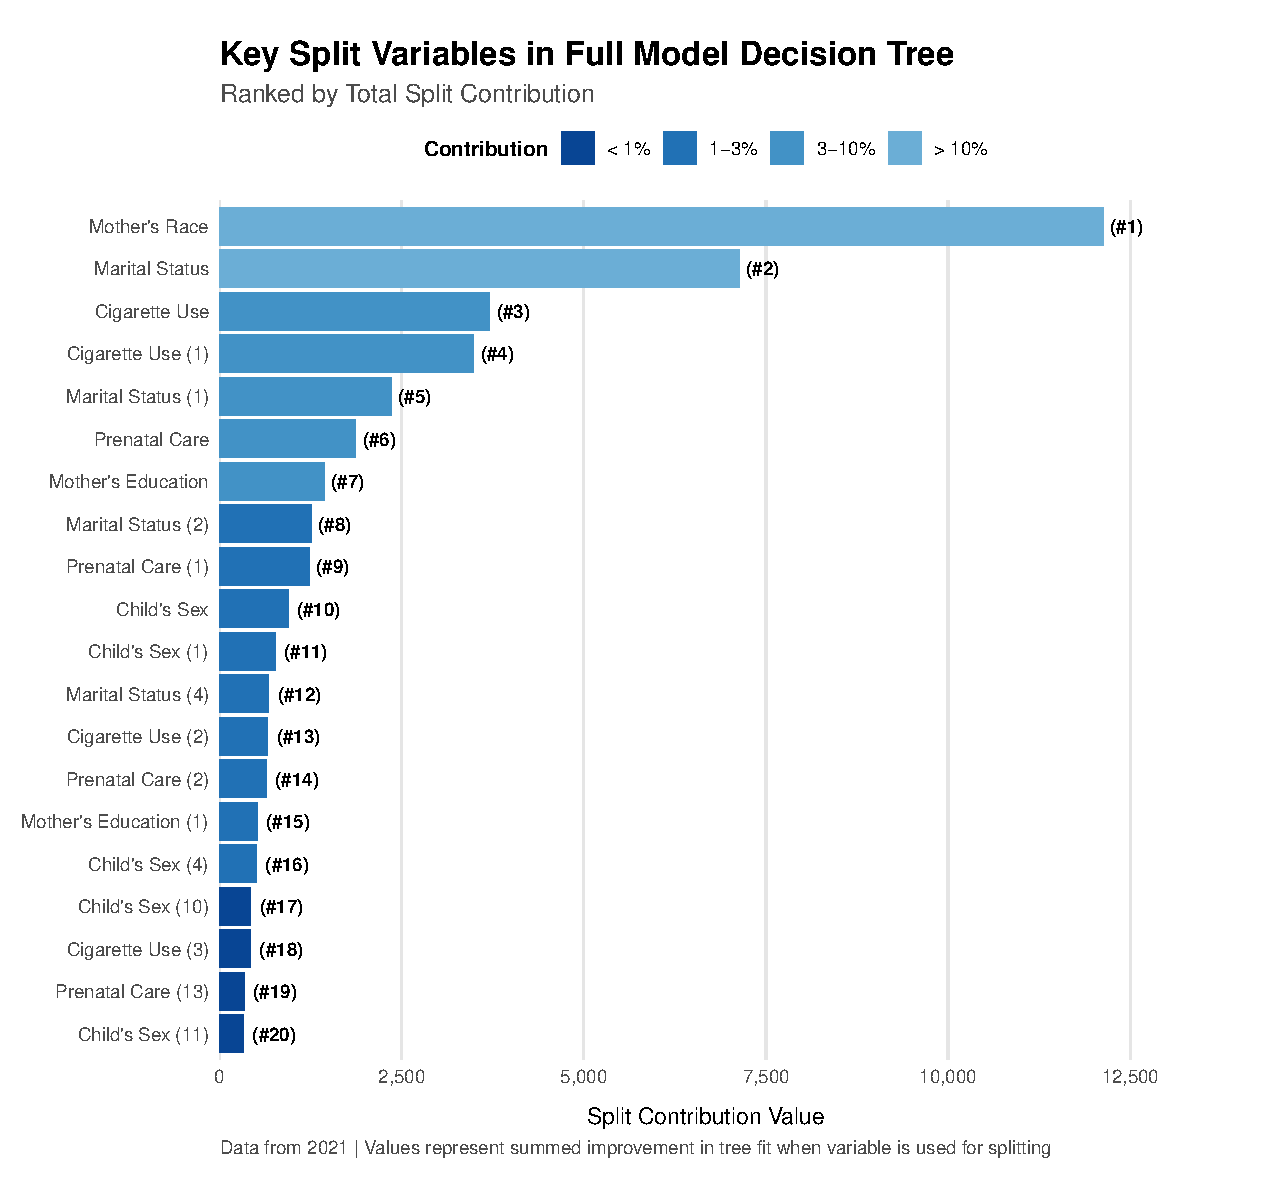
\includegraphics[width=1\linewidth]{chapters/chapter3/figures/improvement/tree_split_contribution_top20_Full Model.pdf}
    \caption{Full Model Ranked Improvement. Rankings represent summed reduction in deviance (improvement in model fit) across all nodes where each variable is used for splitting in the tree. Plot only displays top 20 ranked variables.}
    \label{fig:full-model-ranked-imp}
\end{figure}

% ranked improvement - LBW
\begin{figure}[H]
    \centering
    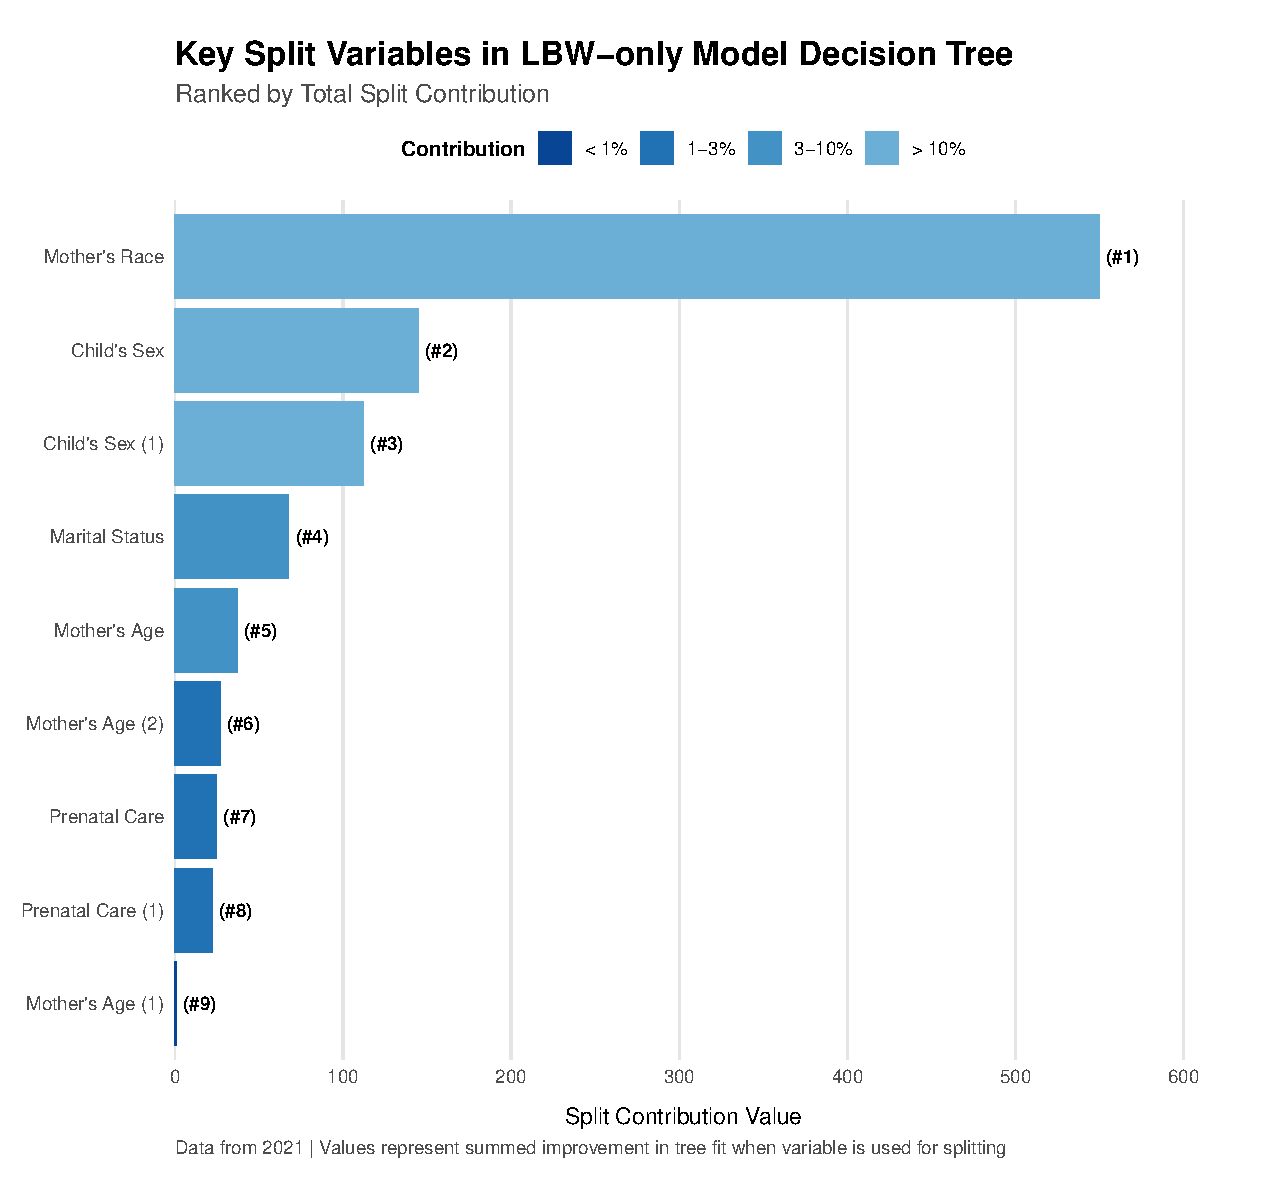
\includegraphics[width=1\linewidth]{chapters/chapter3/figures/improvement/tree_split_contribution_top9_LBW-only Model.pdf}
    \caption{LBW-only Model Ranked Improvement. Rankings represent summed reduction in deviance (improvement in model fit) across all nodes where each variable is used for splitting in the tree. Plot displays all ranked variables.}
    \label{fig:lbw-model-ranked-imp}
\end{figure}

% First barplot figure
\begin{figure}[H]
    \centering
    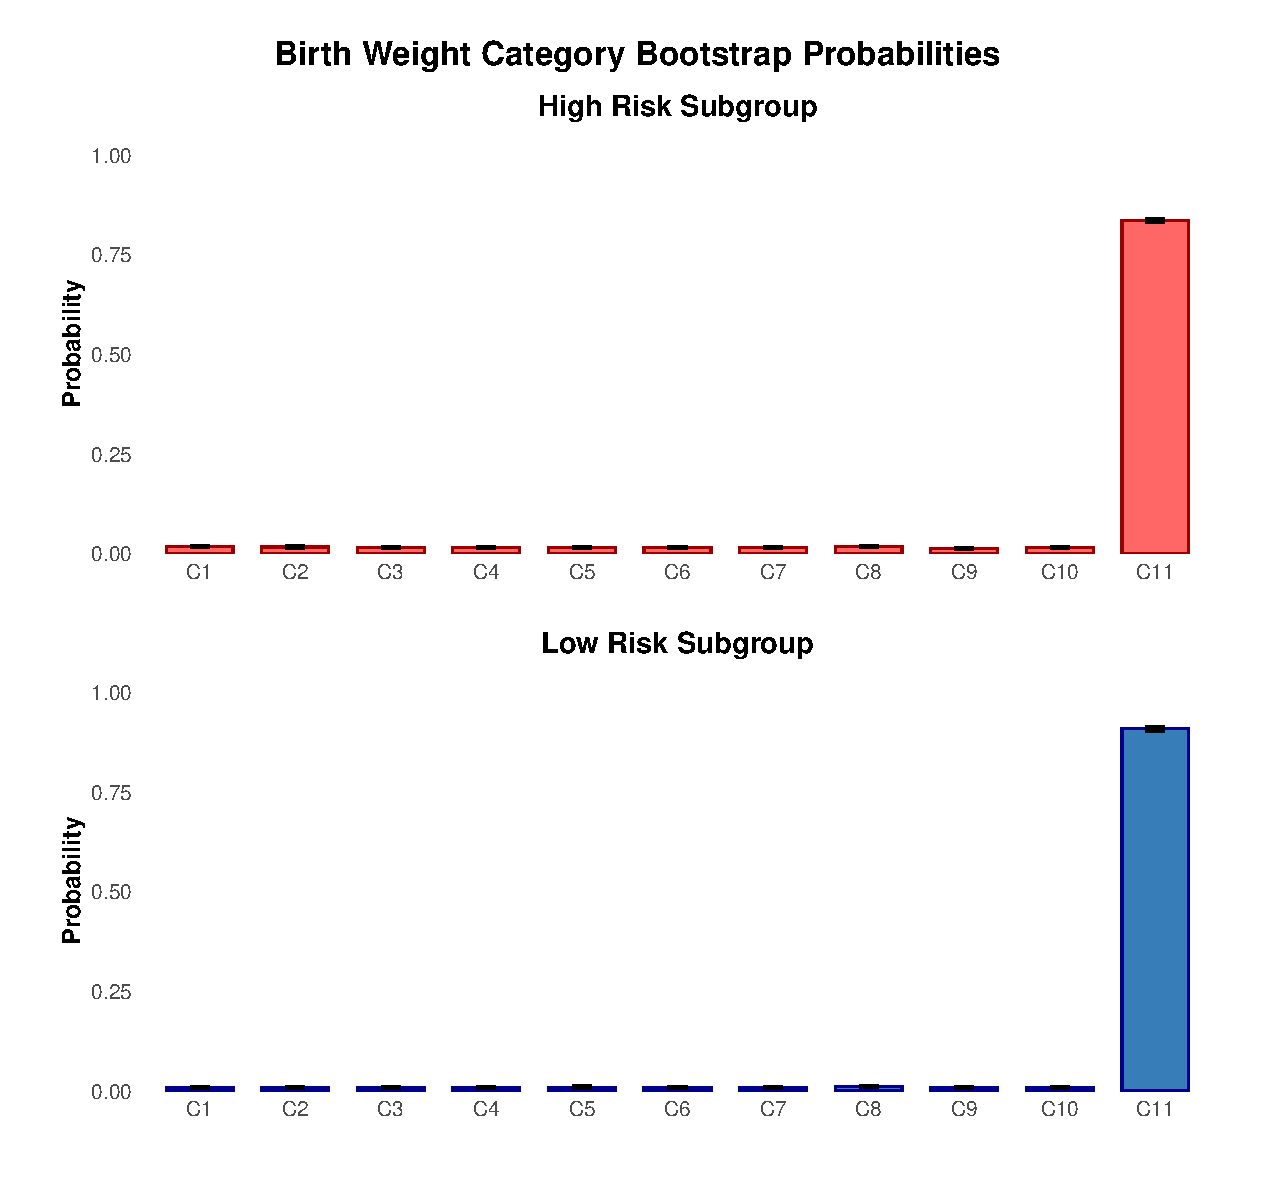
\includegraphics[width=1\textwidth]{chapters/chapter3/figures/high_low_risk_full.pdf}
    \caption{Full model: Aggregated mean probability estimates by birth weight category across $B$ bootstraps, showing the distribution of predicted probabilities for high and low risk subgroups with 95\% confidence intervals.}
    \label{fig:high-low-risk-full}
\end{figure}

% Second barplot figure
\begin{figure}[H]
    \centering
    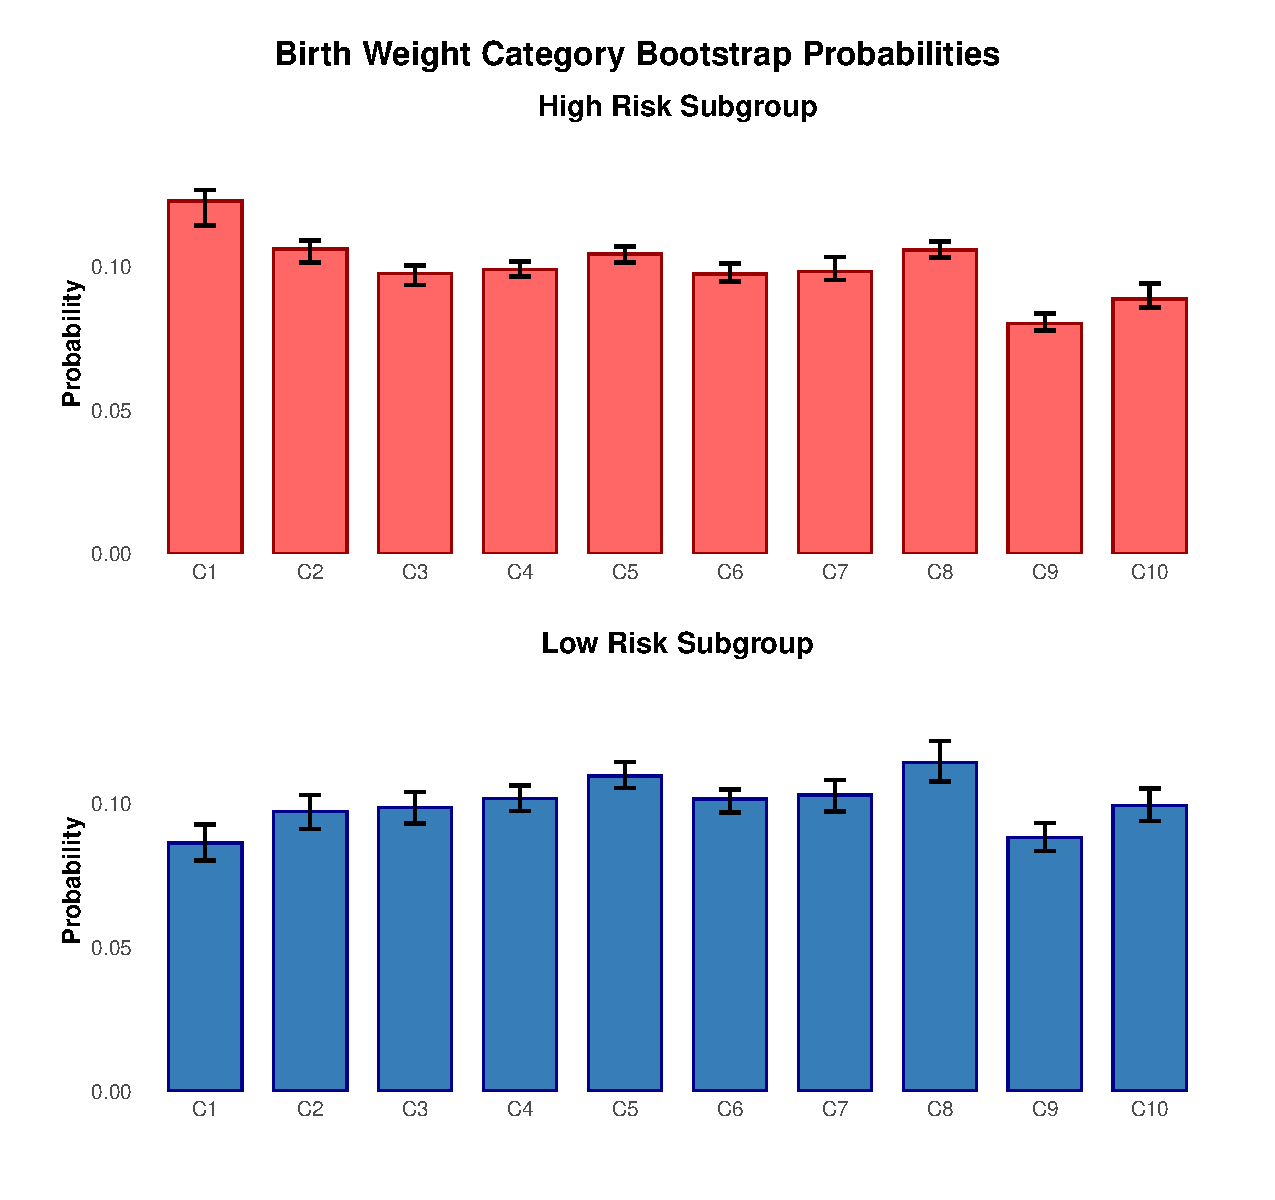
\includegraphics[width=1\textwidth]{chapters/chapter3/figures/high_low_risk_small.pdf}
    \caption{LBW-only model: Aggregated mean probability estimates by birth weight category across $B$ bootstraps, showing the distribution of predicted probabilities for high and low risk subgroups with 95\% confidence intervals.}
    \label{fig:high-low-risk-lbw}
\end{figure}


% Depth distributions — Full model
\begin{figure}[H]
    \centering
    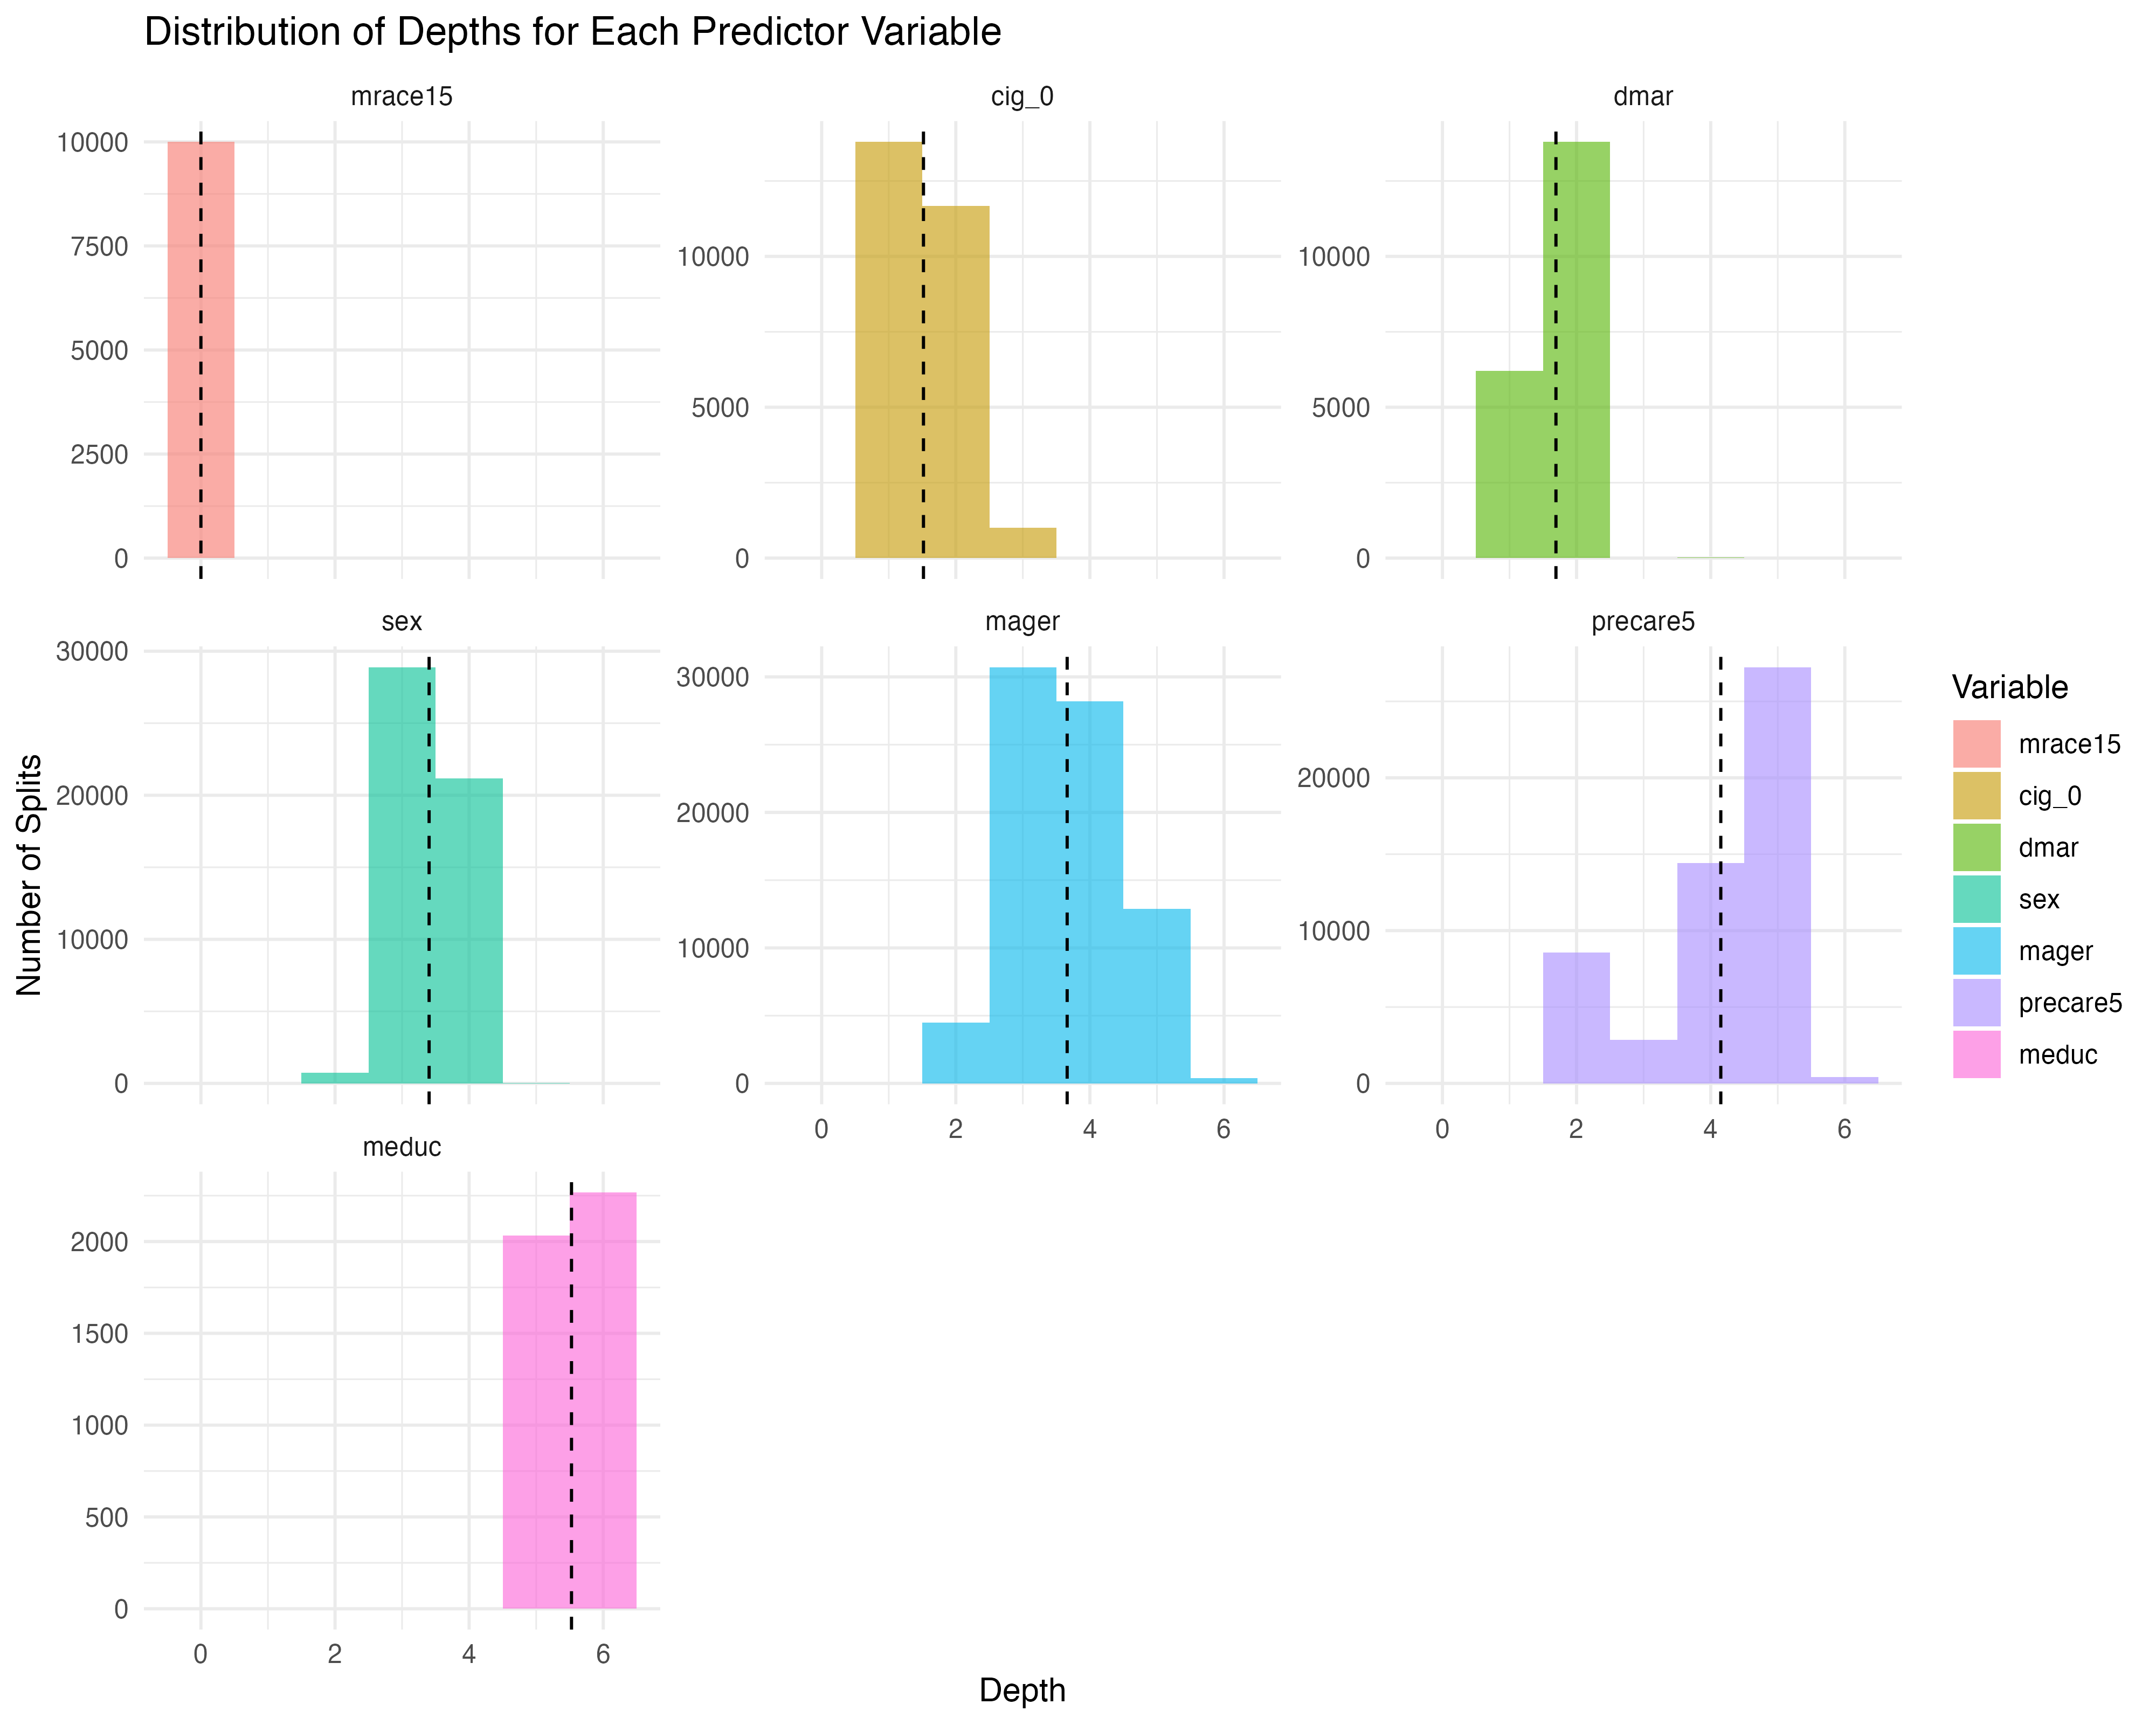
\includegraphics[width=1.0\textwidth]{chapters/chapter3/figures/boot/depth_distributions.png}
    \caption{Full model: Distribution of variable depths across the ensemble. Each panel shows a histogram indicating how frequently a given variable appears at each tree depth, where depth 0 corresponds to the root node. Variables closer to the root are generally more important in the model.}
    \label{fig:var-depth-distributions-full}
\end{figure}

% Depth distributions — LBW-only model
\begin{figure}[H]
    \centering
    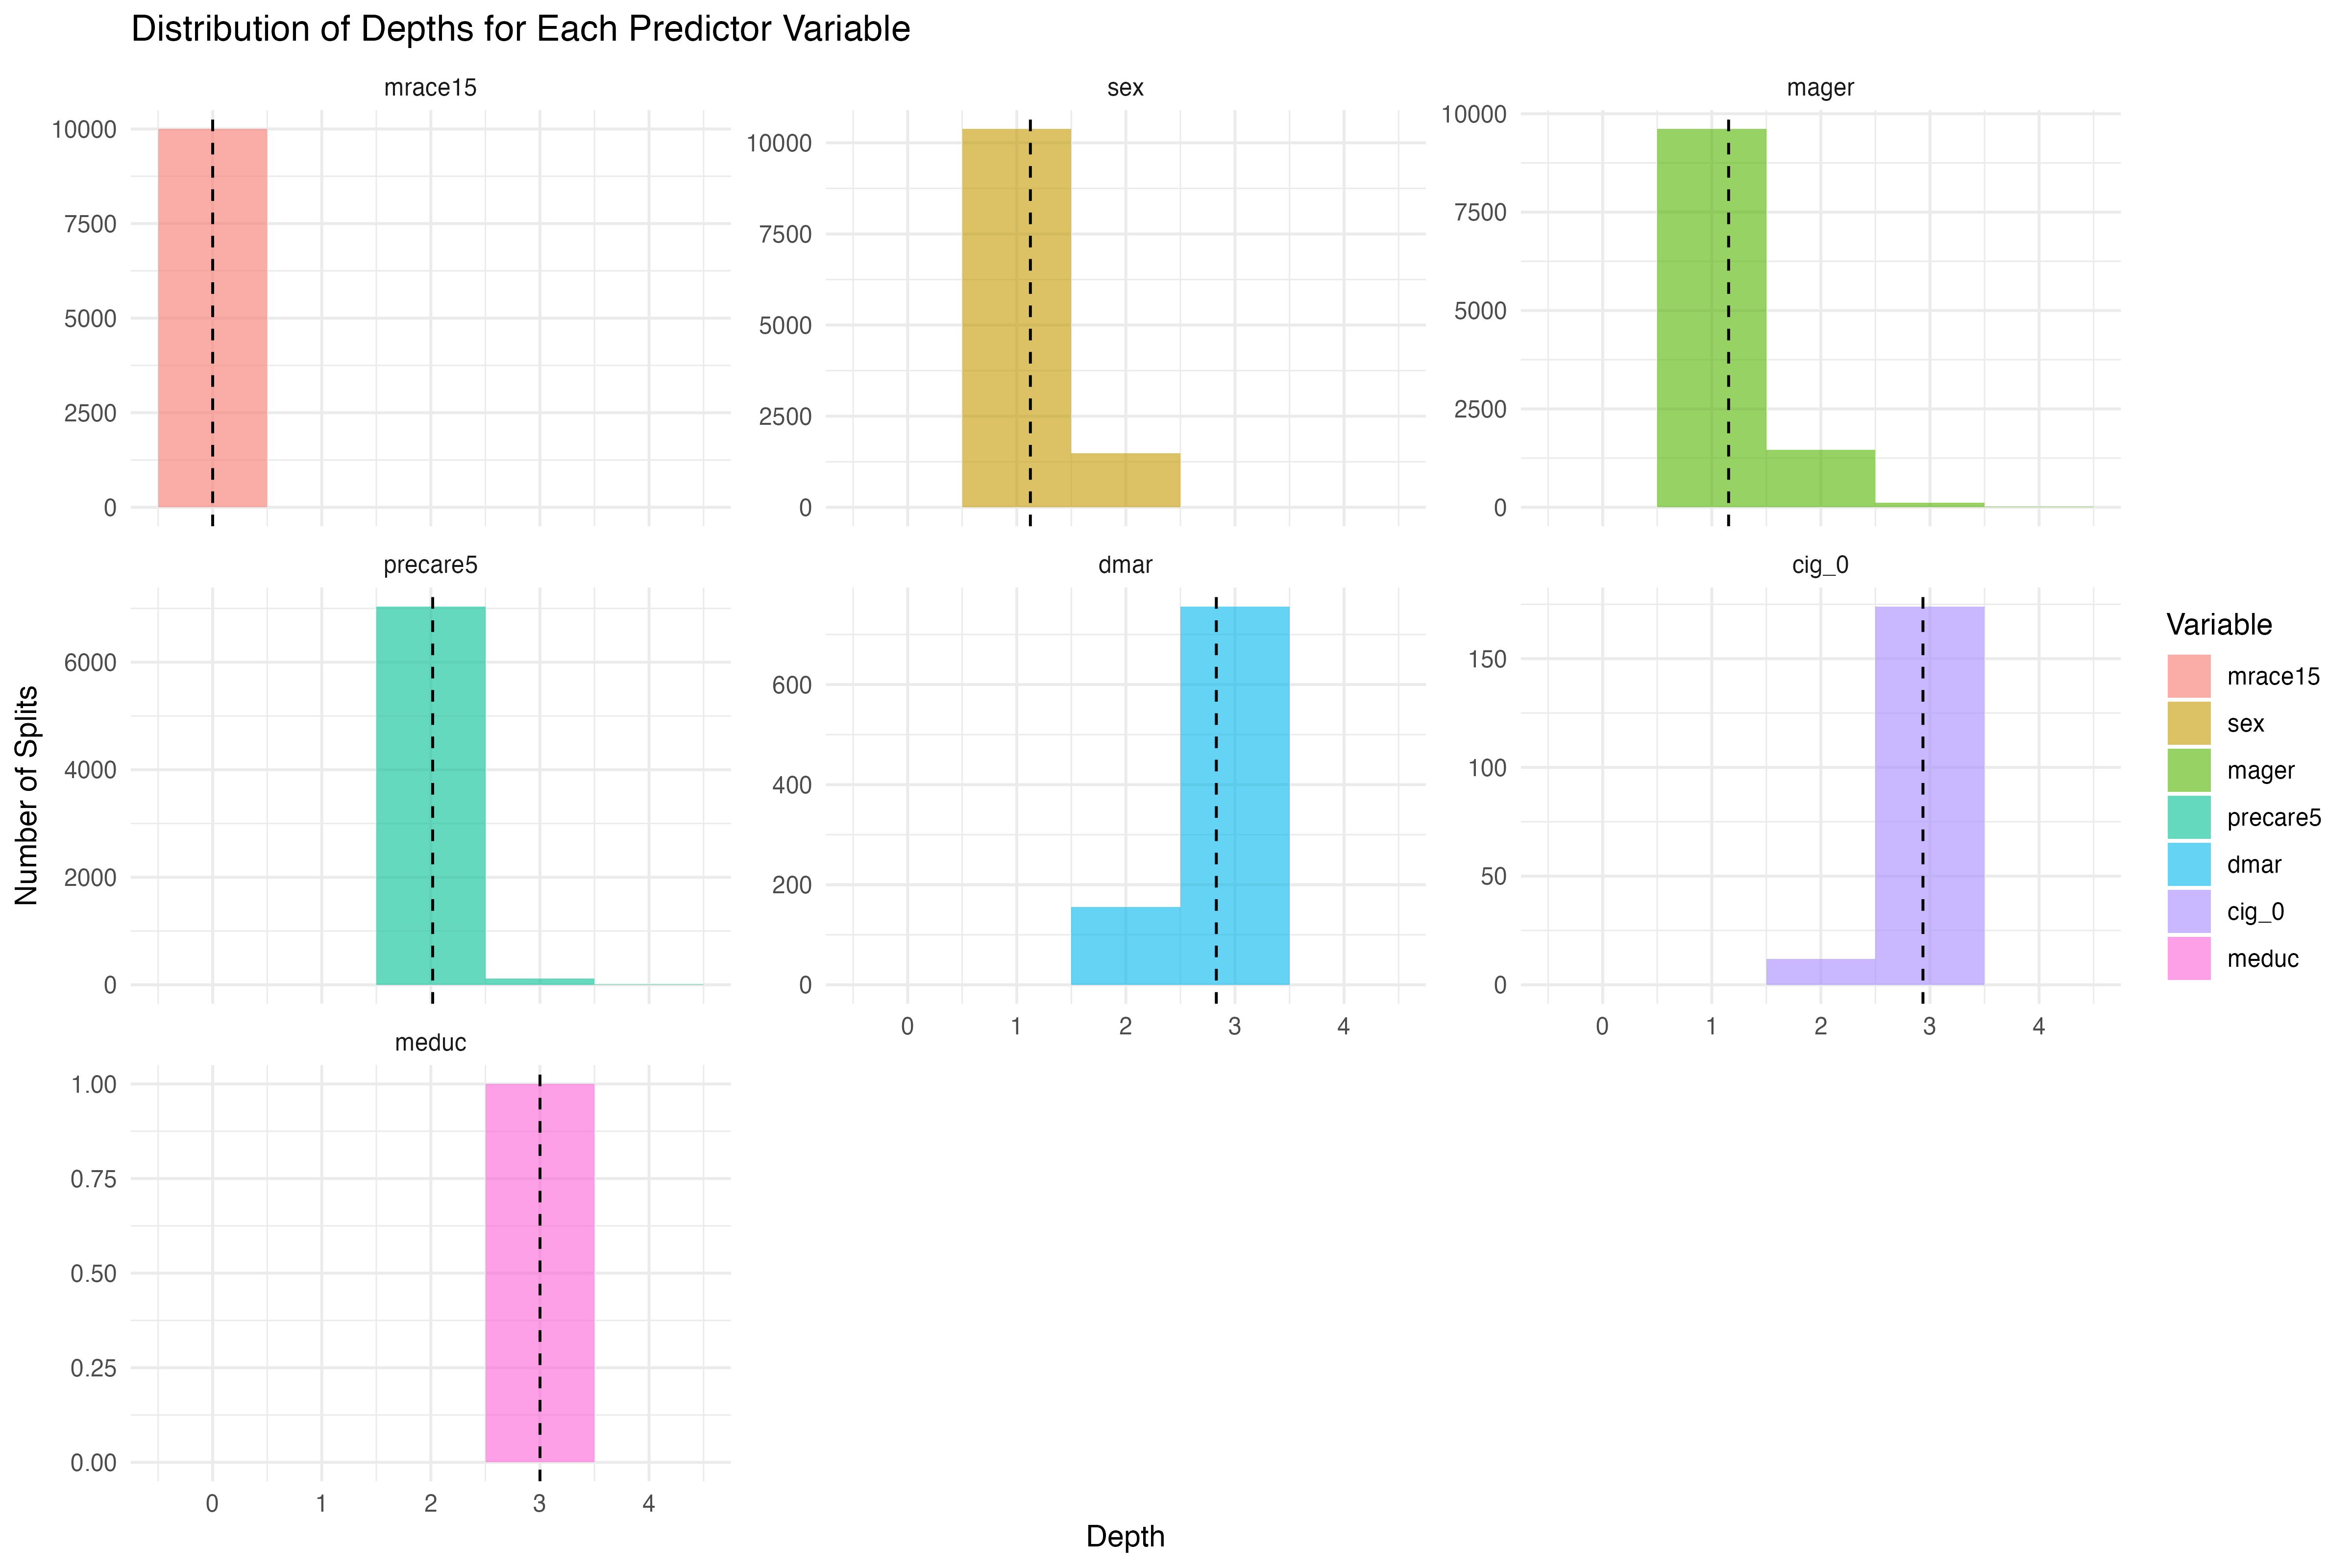
\includegraphics[width=1.0\textwidth]{chapters/chapter3/figures/boot/depth_distributions_2.png}
        \caption{LBW-only model: Distribution of variable depths across the ensemble. Each panel shows a histogram indicating how frequently a given variable appears at each tree depth, where depth 0 corresponds to the root node. Variables closer to the root are generally more important in the model.}
    \label{fig:var-depth-distributions-lbw}
\end{figure}




\chapter{Tree-based Nonparametric Birth-Weight Modeling}
\label{chap:chapter3-title}

% Input individual section files
\section{Previous Work on Birth Weight Modeling}
\label{sec:ch2-previous-work}

As previously mentioned, \textcite{kramer1987}'s \citeyear{kramer1987} meta-analysis identified 43 LBW determinants then categorized them into genetic, nutritional, psychosocial, etc. and assessed their effects on birth weight and prematurity. Separated based on income status, for high-income mothers, smoking status, poor maternal nutrition or low pre-pregnancy weight were the strongest LBW determinants whereas in low-income settings, maternal race origin, undernutrition, short stature, and malaria exposure were found to be the most important predictors \parencite{kramer1987}. While for preterm births, smoking status and low pre-pregnancy weight are strong indicators \parencite{kramer1987}.  \textcite{kramer1987} concluded by stating that many potential contributors remain under-studies, naming maternal work, prenatal care, and previous infections as examples. This comprehensive work highlights the complex and multifactorial nature of LBW, leaving open questions about interactions of factors and distributional outcomes, motivating a more flexible modeling procedure.

The application of CART by \textcite{KITSANTAS2006275} (\citeyear{KITSANTAS2006275}) to 181,690 singleton births from Florida, led the identification of high-risk LBW mothers. Known risk factors of smoking status, gestation weight-gain, parity, etc. were used to grow separate decision trees by geographic region, and compared against logistic regression \parencite{KITSANTAS2006275}. The CART model revealed high-risk profiles for White and Hispanic mothers with low pregnancy weight gain, and parity and marital status defined high-risk stratification among non-smokers \parencite{KITSANTAS2006275}. For instance, smoking mothers gaining less than 20 lbs were at significantly higher risk than larger weight gain, and Black mothers formed high-risk subpopulation in some regions regardless of other factors \parencite{KITSANTAS2006275}. However, predictive accuracy was only marginally better than logistic regression \parencite{KITSANTAS2006275}, the recursive partitioning procedure conducted by CART uncovered some of the complex factor interaction in the LBW data. This study shows how the order of factors could be useful in disentangling strong interaction effects, suggesting room for improved or alternative methods. 

\textcite{dunson2008} (\citeyear{dunson2008}) used Bayesian semiparametric methods to link maternal pregnancy weight gain to birth weight distributions. Using a Dirichlet-process mixture, they flexibly defined clusters of women by their weight-gain trajectories and jointly modeled birth weight densities across clusters \parencite{dunson2008}. This approach allowed the \emph{entire} birth weight distribution to vary with weight-gain patterns, including distribution tails, while also capturing heterogeneity of how pregnancy factors influence birth weigh \parencite{dunson2008}. Dunson et. al. demonstrate that modeling the full distribution in perinatal data is insightful, beyond mean estimates. However, advanced Bayesian models, latent clustering, and complex MCMC procedures lack interpretability and are computationally intensive, highlighting the need for model simplicity while retaining flexibility.

More recently, \textcite{rathjens2023} in \citeyear{rathjens2023} proposed a Bayesian distribution regression approach using copulas to jointly model birth weight and gestational age. Marginal distributions are assumed to follow a normal for birth weight outcomes, and Dagum for skewed gestational age, and the copula linked them as functions of the covariates \parencite{rathjens2023}. The results of this study show non-linear effects of gestational age on weight and tail-dependent associations were captured by Clayton copula \parencite{rathjens2023}. The focus of bivariate outcomes here shows how distribution modeling can extend traditional regression approaches. Beyond complex copula models, Bayesian methods enrich perinatal risk modeling. 

In \citeyear{jain2024}, \textcite{jain2024} proposed a scalable Bayesian density estimation method for nationally collected birth records. Inspired by kernel density methods, a Gaussian mixture is employed to model conditional distributions of birth weights given various predictors. Through advanced MCMC and targeted subsampling techniques, the model was able to capture complex patterns and estimate birth weight densities at scale. Jain's work estimates the full distribution by density regression, but underscores the computational and interpretational challenge involved.

\section{Current Approach \& Contributions}
\label{sec:ch2-current-approach}

In this thesis, we adopt CART and Bayesian nonparametric methods to approximate birth weight distributions. CART is a nonparametric algorithm proposed by \textcite{breiman1984classification} (\citeyear{breiman1984classification}) and implemented in R by Therneau et al. \parencite{intro_to_rpart}, called \textit{Recursive Partitioning and Regression Trees}, or \texttt{rpart}. The algorithm works in two stages: tree construction and tree pruning. 
 
First, the tree is constructed. Given the data, \texttt{rpart} recursively partitions it into binary splits on the given predictor variables, creating nodes at each split. Though the splits need not be binary, this provides a clear and interpretable tree. CART employs a greedy approach to building decision trees \parencite{cart_greedy}, where its goal is to maximize homogeneity, or equivalently minimize heterogeneity in the data. At each node, CART evaluates all possible splits on candidate predictors and chooses the one that best explains the data by minimizing the node impurity, resulting in two child nodes with more homogeneous responses \parencite{intro_to_rpart}. This process is applied recursively to each child node, growing a larger tree until the tree's max depth is reached or no further improvement is found \parencite{intro_to_rpart}.

Once fully grown, the tree typically overfits to the data, yielding large errors for small fluctuations. To address this, cross-validation is used to estimate prediction error for a sequence of pruned trees \parencite{intro_to_rpart}. The tree is then "trimmed" back to the best cross-validation performance \parencite{intro_to_rpart}, yielding the final tree that balances complexity and accuracy. For each terminal node (or "leaf") in the final tree, a sequence of if-then conditions categorize birth weight outcomes based on maternal covariates.

Interpretability is preserved by using CART to automatically uncover high- and low-risk groups for subpopulations of specific maternal and infant characteristics, much akin to \textcite{KITSANTAS2006275}. Additionally, in line with \textcite{dunson2008} and \textcite{jain2024}, this tree-based method imposes no strict distributional assumptions on the birth weight responses allowing for nonlinear interactions and heterogeneous effects to be captured naturally by CART. Our preprocessing procedure results in count data of various birth weight categories, motivating the use of the \emph{marginal Dirichlet-Multinomial (DM) likelihood} as the Bayesian "evidence" and splitting criterion. The DM likelihood is chosen by producing posterior predictive distributions and interval estimation at each leaf whereas the Gini index measures only impurity. The impurity of a terminal node, is entirely dependent on the sample size by relying on empirical proportions \parencite{stackexchangeGiniDecrease}. Additionally, the Gini index is known to suffer with data sparsity \parencite{ekamperiDecisionTrees}, and compared to normal birth weight (NBW) observations, we expect a large discrepancy between the total number of observed LBW and NBW counts.

Birth weight counts observations can be safely assumed to follow a multinomial distribution, and the Dirichlet prior smooths categories not observed in the sample. For use in CART, a split with high DM likelihood translates as added improvement from parent to child nodes, reducing heterogeneity. The DM likelihood will be derived formally in Section~\ref{sec:ch2-likelihood} as a favorable splitting criterion for our application.

 \section{Overview of the Birth Weight Dataset}
\label{sec:ch2-introduction}
%Description of 2021 Vital Statistics Natality Birth Data
%Key demographic, health, and geographic variables
%Challenges due to large dataset size and skewed LBW distribution

The primary dataset for this analysis is the 2021 Vitality Statistics Natality Birth Data \parencite{nber_birth_data}. Collected by the National Center for Health Statistics (NCHS), this dataset contains a detailed record of birth outcomes and various maternal characteristics as part of the Vital Statistics Cooperative Program \parencite{jain2024, nber_birth_data}. Standing as one of the most comprehensive datasets with over 3 million birth weight records for maternal and infant health in the United States, collected annually across all states and District of Columbia since 1972 \parencite{nber_birth_data}.

For this analysis, variables in the 2021 data are broadly categorized into three domains: demographic, health, and geographic. Demographic features include date of birth, parental age and education, marital status, birth order, sex, and geographic location. Health features cover birth weight, gestational age, prenatal care adequacy, delivery attendants, and Apgar scores, and geographic indicators include state, county, and metropolitan  status \parencite{nber_birth_data}. Note that Apgar examinations examine newborn vitals five minutes after birth, observing how the newborns are handling being outside the mother's womb  \parencite{apgar_score}. 

\section{Data Preprocessing \& Feature Engineering}
\label{sec:ch2-preprocessing}

The preprocessing procedure transforms the high-dimensional 2021 dataset into a workable and condensed dataset for computational efficiency, while preserving key information about predictors. Preprocessing involved (1) encoding all categorical and continuous variables into unique dichotomous predictors, (2) dimension reduction from 3 million rows to 128 unique predictor combinations, and (3) creating a consolidated counts dataset, primarily expanding the LBW region by creating birth weight categories based on quantile cut-points. From the dataset, seven key predictor variables and birth weight outcomes (in kg) are retained for modeling. 

\subsection{Binary Feature Encoding}
\label{sec:ch2-feature-encoding}

To enhance interpretability and computational efficiency, only seven predictors are selected based on clinical relevance, strong generalizability,  and prior research support. The encoding procedure was inherited from \textcite{jain2024}, and these predictors serve as an example of a small, yet representative set of predictors. Note that the encoding of \texttt{mrace15} is suggested by \textcite{jain2024, marchofdimes2024} as the primary dichotomy, \emph{though this choice is entirely arbitrary}.  According to \citeyear{census_usa} \textcite{census_usa} estimates, the national population is roughly 75.3\% White and 13.7\% Black, which provides demographic context for this binary split. All information of each feature representation and meaning is conveyed in the table below.

\begin{table}[ht]
\centering         % ensures horizontal centering
\small             % or \footnotesize
\caption{Binary predictor definitions used in this study}
\begin{tabular}{@{}llll@{}}
\toprule
\textbf{Label} & \textbf{Natality field} & \textbf{Value = 1} & \textbf{Value = 0} \\ \midrule
Boy          & \texttt{sex}      & Infant is male (“M”)                     & Infant is female (“F”) \\
Married      & \texttt{dmar}     & Mother is married                        & Mother not married     \\
Black        & \texttt{mrace15}  & Black / African American                 & Any other race         \\
Over33       & \texttt{mager}    & Maternal age $>$ 33 yr                   & Maternal age $\le$ 33 yr \\
HighSchool   & \texttt{medu}     & High-school education completed          & Otherwise              \\
FullPrenatal & \texttt{prenatal} & Adequate prenatal care                   & Inadequate / none      \\
Smoker       & \texttt{cig\_0}   & Any prenatal smoking                     & No smoking             \\ \bottomrule
\end{tabular}
\end{table}



\subsection{Dimension Reduction}
\label{sec:ch2-dimension-reduction}

After the first step in preprocessing, the data is encoded as dichotomous indicator variables and one response column of total recorded birth weight outcomes for the 3 million rows. There are \(2^7 = 128\) possible combinations for the predictors, each representing a unique class of maternal and infant characteristics. Aggregating observations by class greatly reduces the computational load while preserving interpretability, and necessary information of features, enabling discernment of risk factors with minimal computational burden.

\subsection{Converting Birth Weight into Count Variables} 
\label{sec:ch2-count-variables}

The final step, transforms the dataset from 3.6 million by 237 to 128 by 11. We define a sequence of decline-quantile cut-points based on 10\% quantile increments, to segment the LBW region from 0-to-2.5 kg creating 10 total LBW categories. By using the previous year's identical dataset from 2020 in segmenting these categories, we eliminate problems with "double-dipping" and bias in later estimates. This dimension reduction drastically consolidates the dataset while providing a straightforward way to retrieve a given number of birth weight counts of a given class and quantile. The specific cut-point values and their prior assignment are shown in the following table:

% insert table of quantile cut-points
\begin{table}[htbp]
\centering
\caption{Birth-weight quantile cut points and Dirichlet priors}
\label{tab:birthweight_quantiles}
% siunitx is needed only for the S columns
\begin{tabular}{@{}l c S[table-format=2.2] c S[table-format=2.2]@{}}
\toprule
& \multicolumn{2}{c}{\textbf{Type 1: LBW + Normal}} &
  \multicolumn{2}{c}{\textbf{Type 2: LBW only}} \\
\cmidrule(lr){2-3}\cmidrule(lr){4-5}
\textbf{Quantile} &
  \textbf{Range (g)} & {\textbf{Prior (\%)}} &
  \textbf{Range (g)} & {\textbf{Prior (\%)}} \\
\midrule
Q1     &  227--1170 & 0.84 &  227--1170 & 10 \\
Q2     & 1170--1644 & 0.84 & 1170--1644 & 10 \\
Q3     & 1644--1899 & 0.83 & 1644--1899 & 10 \\
Q4     & 1899--2069 & 0.83 & 1899--2069 & 10 \\
Q5     & 2069--2183 & 0.87 & 2069--2183 & 10 \\
Q6     & 2183--2270 & 0.83 & 2183--2270 & 10 \\
Q7     & 2270--2350 & 0.86 & 2270--2350 & 10 \\
Q8     & 2350--2410 & 0.93 & 2350--2410 & 10 \\
Q9     & 2410--2460 & 0.71 & 2410--2460 & 10 \\
Q10    & 2460--2500 & 0.80 & 2460--2500 & 10 \\
Normal & \textgreater{}2500 & 91.67 & & \\
\bottomrule
\end{tabular}
\end{table}

As seen in Table~\ref{tab:birthweight_quantiles} the two types include: low and normal birth weights (NBW), and the other restricted to LBW, where NBW is defined as any birth weight observation greater than 2.5 kg \parencite{wiki:nbw}. Once the tree is fit, they are called the "full" and "LBW-only" models respectively. The NBW observations are aggregated into one column called \texttt{counts\_above\_2.5kg}, and will serve as the eleventh birth weight category in the consolidated counts dataset. When given to CART, it is of primary concern how the inclusion of this column changes the tree construction, variable selection, and stability of estimates. Additionally, the prior construction is heavily skewed for the low and NBW with probability of 91.67\%, while the second is a uniform 10\% prior probability across all 10 LBW categories by construction.

In summary, this preprocessing consolidation yields 10 discretized quantile birth weight categories used to allocate all observations into counts. This provides a detailed gradations of the LBW region, and adding the aggregated NBW category provides the full range in the dataset. This approach prevents scarcity in any one category, and the data will be called \emph{counts data} from here forward. 
% \input{chapters/chapter3/bootstrap}
% \input{chapters/chapter3/results}

% Input tables and figures
% Tables
\begin{table}[H]
\centering
\caption{Comparison of Variable Importance in Full Model and LBW-Only Model}
\label{tab:var_comparison}
\begin{tabular}{lcc}
\toprule
& \multicolumn{1}{c}{Full Model} & \multicolumn{1}{c}{LBW-Only Model} \\
\cmidrule(lr){2-2} \cmidrule(lr){3-3}
\multicolumn{3}{l}{\textit{Initial Split Variable}} \\
\midrule
mrace15 & 1.0000 & 1.0000 \\
\midrule
\multicolumn{3}{l}{\textit{Variable Frequency}} \\
\midrule
sex & 1.0000 & 1.0000 \\
dmar & 1.0000 & 0.0915 \\
mrace15 & 1.0000 & 1.0000 \\
mager & 1.0000 & 0.9741 \\
precare5 & 1.0000 & 0.6351 \\
cig\_0 & 1.0000 & 0.0196 \\
meduc & 0.3794 & 0.0000 \\
\bottomrule
\multicolumn{3}{p{0.8\textwidth}}{\textit{Note:} The table shows variable frequency (proportion of trees containing each variable) and initial split variable (normalized measure of predictive contribution) for both models.} \\
\end{tabular}
\end{table}

% ---------------------------  FULL MODEL ---------------------------
\begin{table}[H]
\centering
\caption{Mean probability estimates $\hat{\pi}_{i,k}$ (with 95\% bootstrap percentile intervals) for high‑ and low‑risk birth‑weight subgroups under the \emph{full} model.}
\label{tab:pi_mean_full}
\begin{tabular}{ccccccc}
\toprule
\multirow{2}{*}{Category $k$} & \multicolumn{3}{c}{High‑risk} & \multicolumn{3}{c}{Low‑risk} \\
\cmidrule(lr){2-4}\cmidrule(lr){5-7}
 & $\hat{\pi}$ & 2.5\% & 97.5\% & $\hat{\pi}$ & 2.5\% & 97.5\% \\
\midrule
1  & 1.90 \% & 0.0180 & 0.0202 & 0.80 \% & 0.0075 & 0.0088 \\
2  & 1.72 \% & 0.0163 & 0.0181 & 0.86 \% & 0.0080 & 0.0096 \\
3  & 1.58 \% & 0.0150 & 0.0166 & 0.88 \% & 0.0080 & 0.0100 \\
4  & 1.63 \% & 0.0156 & 0.0170 & 0.90 \% & 0.0083 & 0.0102 \\
5  & 1.69 \% & 0.0162 & 0.0176 & 0.98 \% & 0.0090 & 0.0112 \\
6  & 1.61 \% & 0.0154 & 0.0168 & 0.91 \% & 0.0087 & 0.0098 \\
7  & 1.63 \% & 0.0157 & 0.0170 & 0.93 \% & 0.0088 & 0.0101 \\
8  & 1.78 \% & 0.0172 & 0.0185 & 1.08 \% & 0.0102 & 0.0117 \\
9  & 1.32 \% & 0.0126 & 0.0138 & 0.81 \% & 0.0075 & 0.0090 \\
10 & 1.52 \% & 0.0146 & 0.0158 & 0.96 \% & 0.0089 & 0.0106 \\
11 & 83.62 \% & 0.8330 & 0.8391 & 90.92 \% & 0.9026 & 0.9132 \\
\bottomrule
\multicolumn{7}{p{0.9\textwidth}}{\textit{Note:} $\hat{\pi}$ values are reported as percentages; confidence‑limit columns remain on the \([0,1]\) scale.  Estimates are based on $B$ bootstrap replicates.}\\
\end{tabular}
\end{table}


% ------------------------  LBW‑ONLY MODEL --------------------------
\begin{table}[H]
\centering
\caption{Mean probability estimates $\hat{\pi}_{i,k}$ (with 95\% bootstrap percentile intervals) for high‑ and low‑risk birth‑weight subgroups under the \emph{LBW‑only} model.}
\label{tab:pi_mean_lbw}
\begin{tabular}{ccccccc}
\toprule
\multirow{2}{*}{Category $k$} & \multicolumn{3}{c}{High‑risk} & \multicolumn{3}{c}{Low‑risk} \\
\cmidrule(lr){2-4}\cmidrule(lr){5-7}
 & $\hat{\pi}$ & 2.5\% & 97.5\% & $\hat{\pi}$ & 2.5\% & 97.5\% \\
\midrule
1  & 12.28 \% & 0.1143 & 0.1267 & 8.63 \% & 0.0802 & 0.0928 \\
2  & 10.61 \% & 0.1014 & 0.1090 & 9.73 \% & 0.0911 & 0.1030 \\
3  & 9.75 \% & 0.0935 & 0.1003 & 9.87 \% & 0.0930 & 0.1041 \\
4  & 9.90 \% & 0.0965 & 0.1018 & 10.18 \% & 0.0974 & 0.1064 \\
5  & 10.43 \% & 0.1014 & 0.1069 & 10.96 \% & 0.1054 & 0.1145 \\
6  & 9.74 \% & 0.0948 & 0.1011 & 10.16 \% & 0.0970 & 0.1050 \\
7  & 9.83 \% & 0.0953 & 0.1033 & 10.30 \% & 0.0973 & 0.1082 \\
8  & 10.57 \% & 0.1031 & 0.1088 & 11.42 \% & 0.1078 & 0.1218 \\
9  & 8.01 \% & 0.0776 & 0.0837 & 8.81 \% & 0.0835 & 0.0933 \\
10 & 8.87 \% & 0.0858 & 0.0941 & 9.94 \% & 0.0940 & 0.1053 \\
\bottomrule
\multicolumn{7}{p{0.9\textwidth}}{\textit{Note:} $\hat{\pi}$ values are reported as percentages; confidence‑limit columns remain on the \([0,1]\) scale.  Estimates are based on $B$ bootstrap replicates.}\\
\end{tabular}
\end{table}
% Figures

% ranked improvement - FULL
\begin{figure}[H]
    \centering
    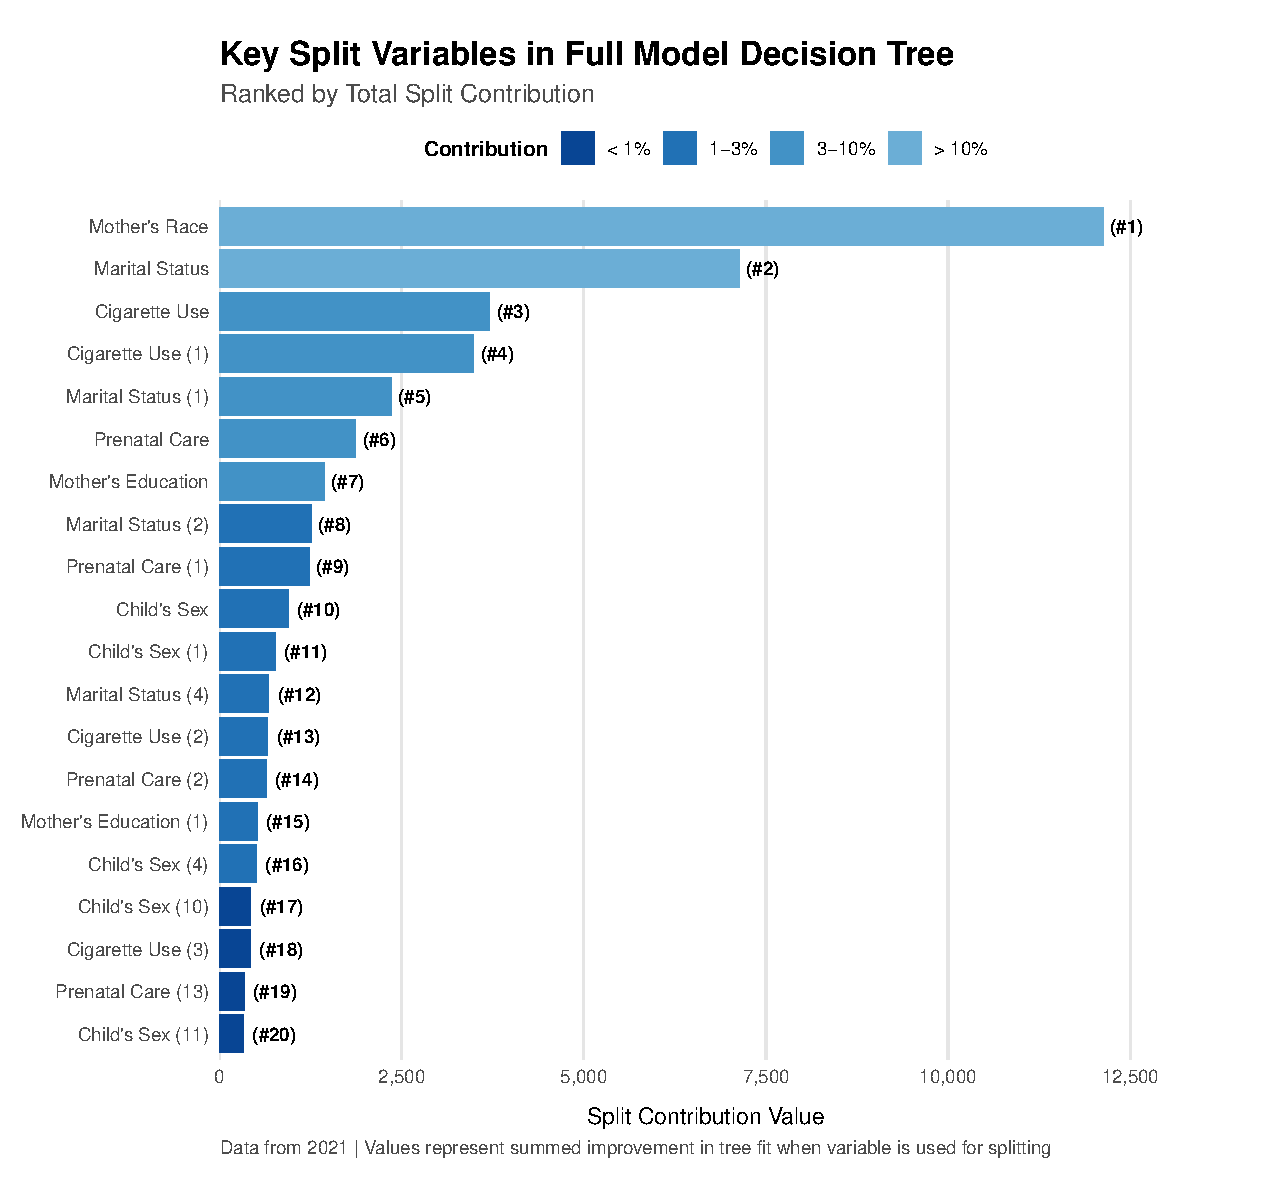
\includegraphics[width=1\linewidth]{chapters/chapter3/figures/improvement/tree_split_contribution_top20_Full Model.pdf}
    \caption{Full Model Ranked Improvement. Rankings represent summed reduction in deviance (improvement in model fit) across all nodes where each variable is used for splitting in the tree. Plot only displays top 20 ranked variables.}
    \label{fig:full-model-ranked-imp}
\end{figure}

% ranked improvement - LBW
\begin{figure}[H]
    \centering
    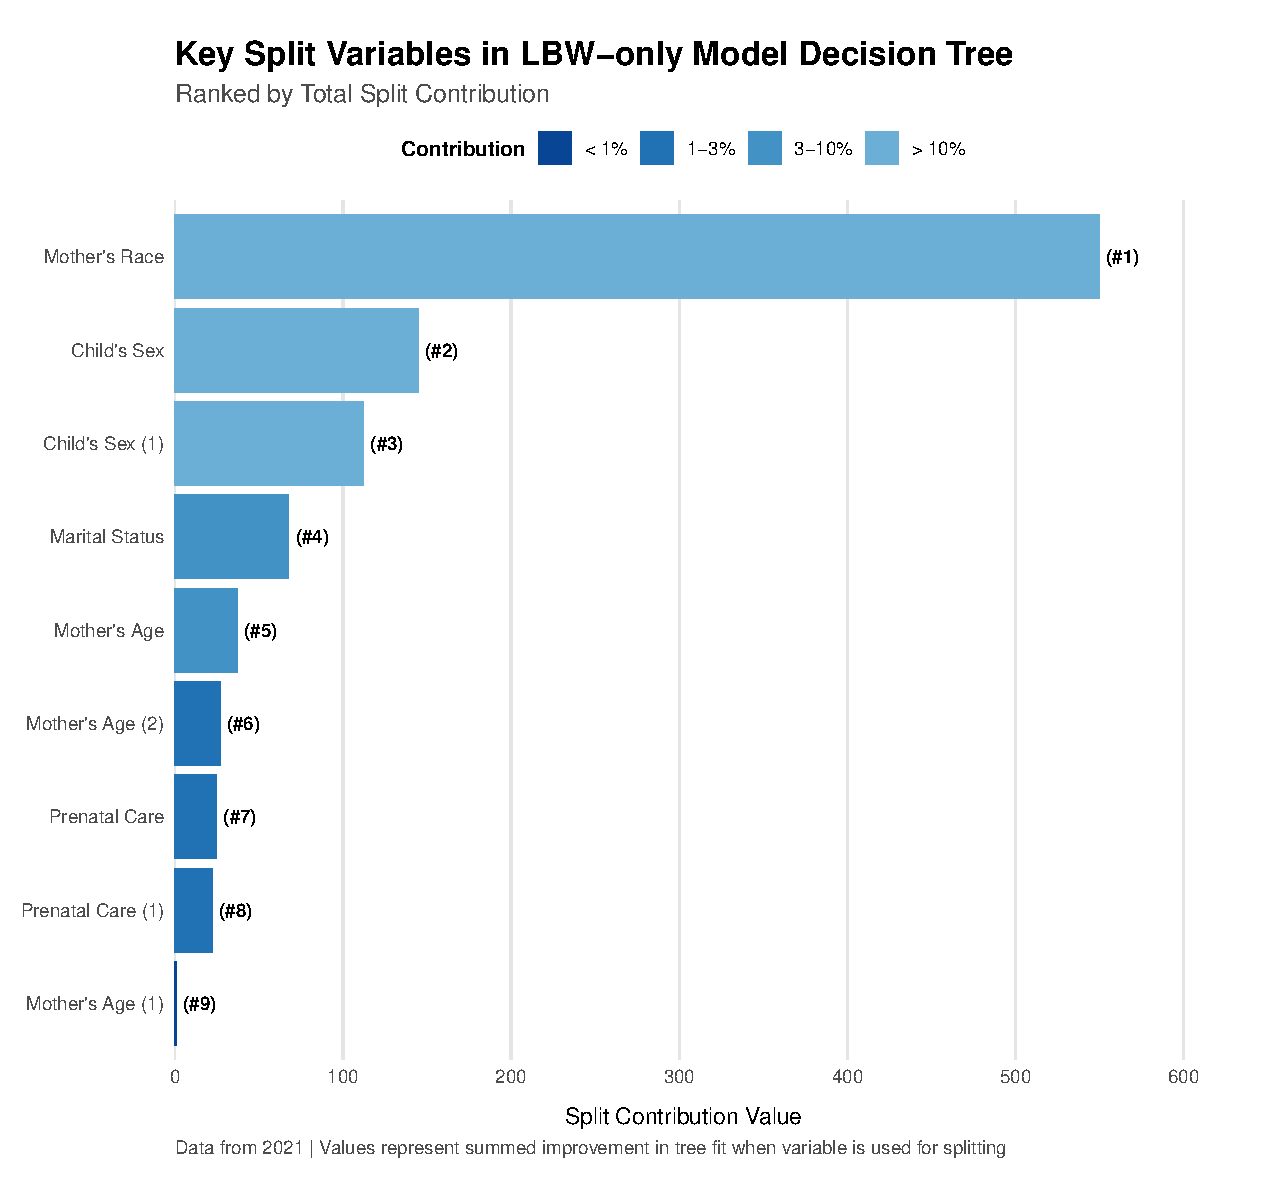
\includegraphics[width=1\linewidth]{chapters/chapter3/figures/improvement/tree_split_contribution_top9_LBW-only Model.pdf}
    \caption{LBW-only Model Ranked Improvement. Rankings represent summed reduction in deviance (improvement in model fit) across all nodes where each variable is used for splitting in the tree. Plot displays all ranked variables.}
    \label{fig:lbw-model-ranked-imp}
\end{figure}

% First barplot figure
\begin{figure}[H]
    \centering
    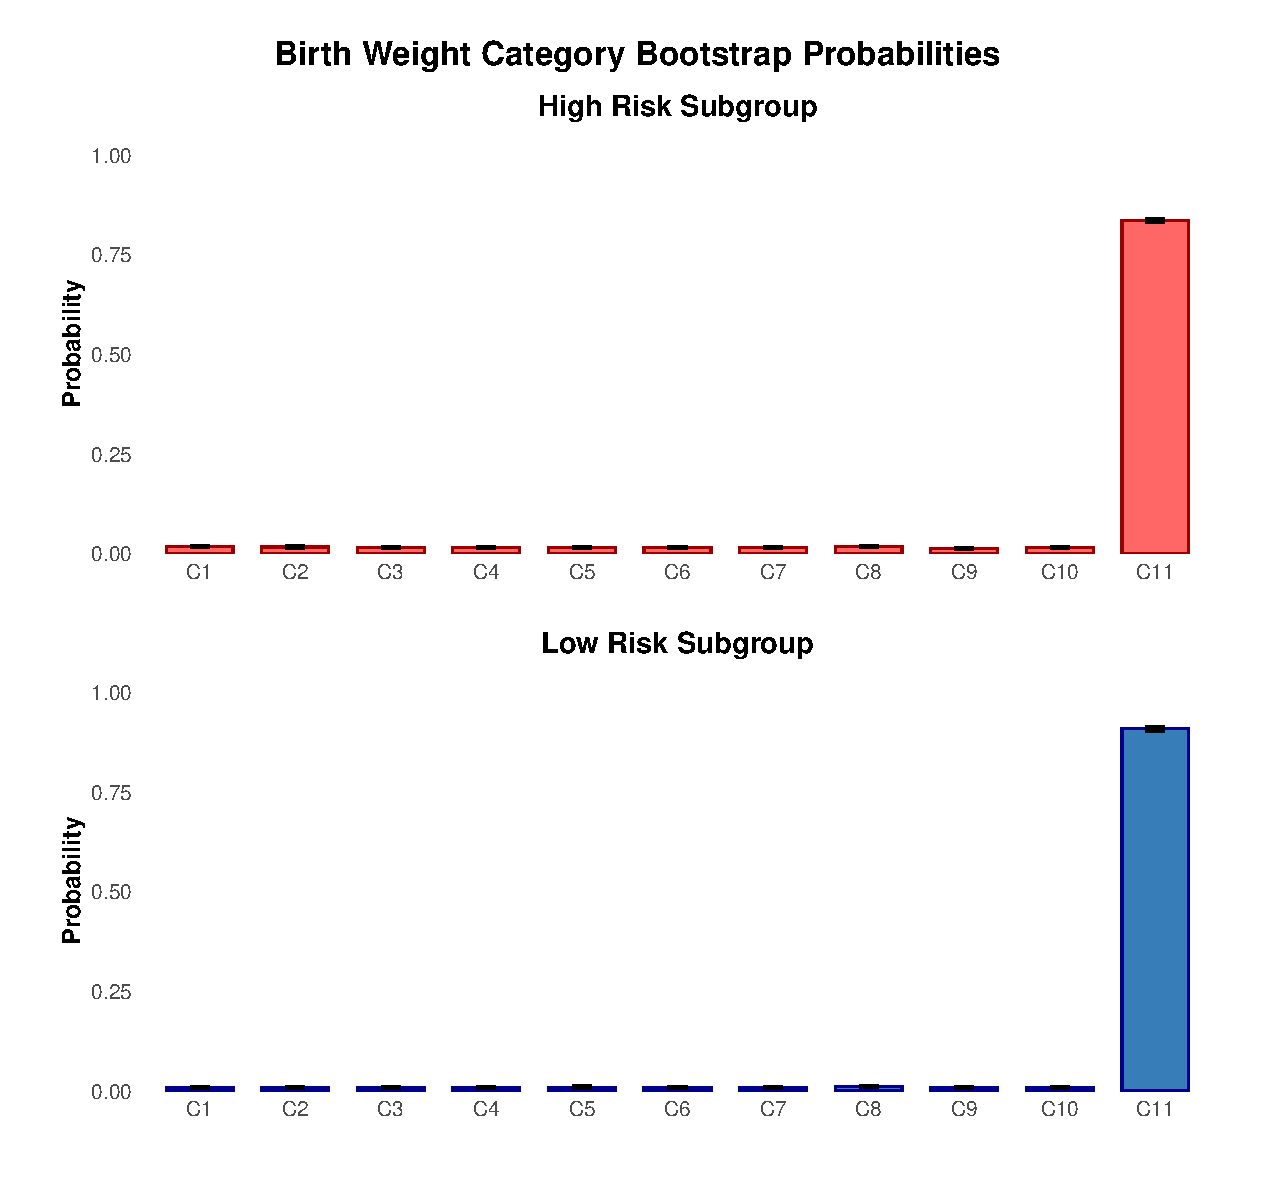
\includegraphics[width=1\textwidth]{chapters/chapter3/figures/high_low_risk_full.pdf}
    \caption{Full model: Aggregated mean probability estimates by birth weight category across $B$ bootstraps, showing the distribution of predicted probabilities for high and low risk subgroups with 95\% confidence intervals.}
    \label{fig:high-low-risk-full}
\end{figure}

% Second barplot figure
\begin{figure}[H]
    \centering
    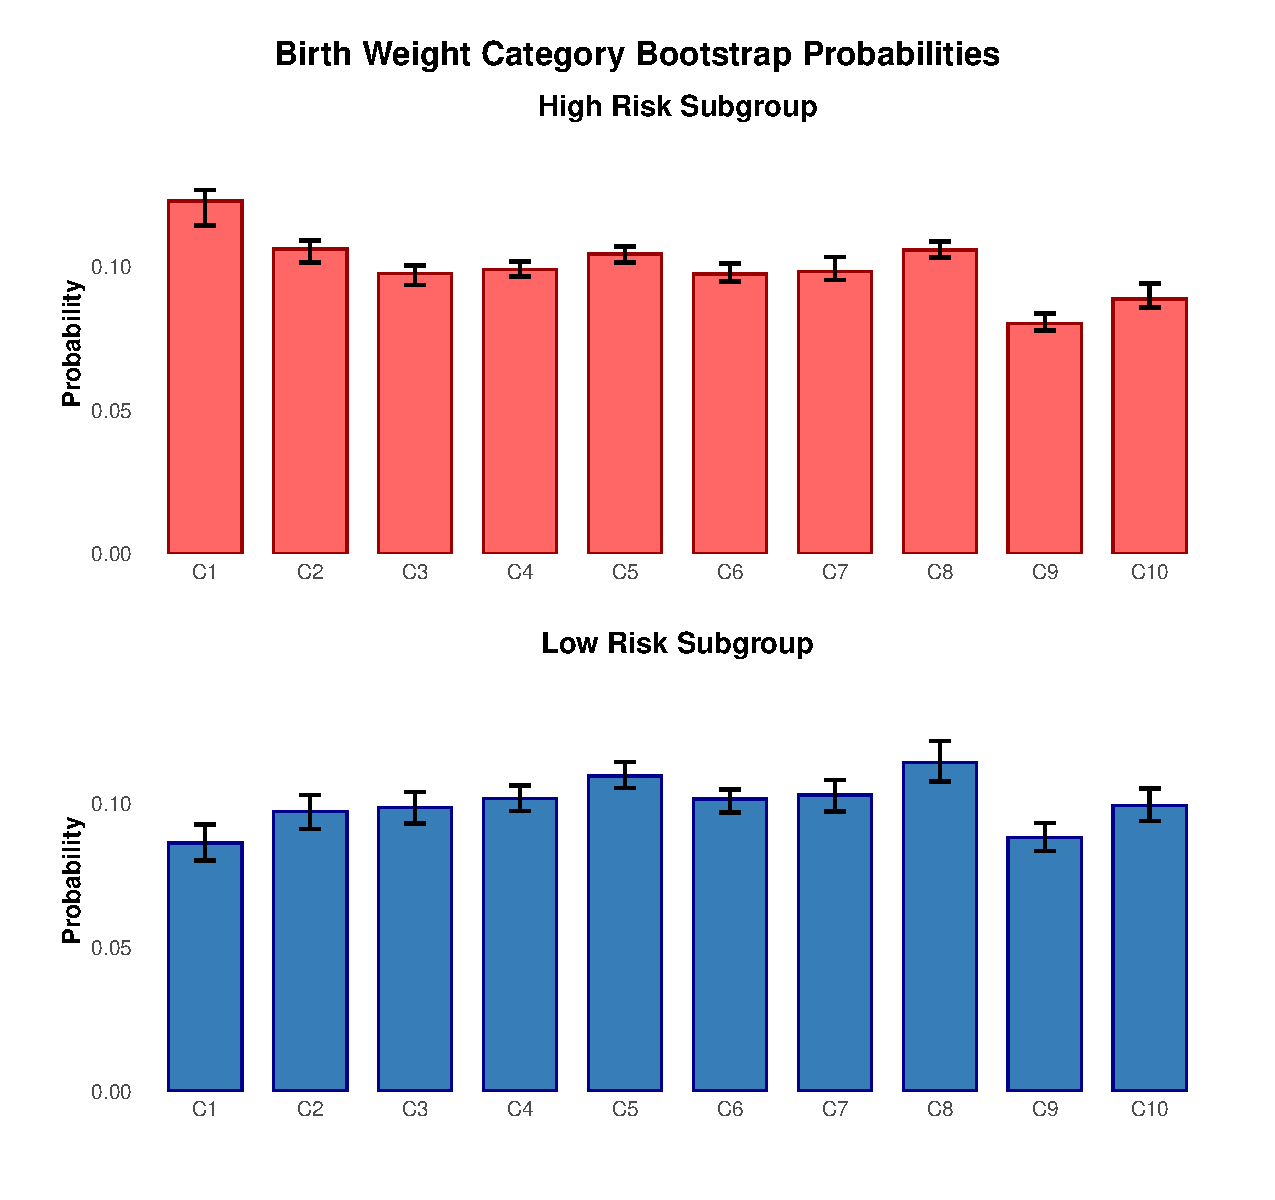
\includegraphics[width=1\textwidth]{chapters/chapter3/figures/high_low_risk_small.pdf}
    \caption{LBW-only model: Aggregated mean probability estimates by birth weight category across $B$ bootstraps, showing the distribution of predicted probabilities for high and low risk subgroups with 95\% confidence intervals.}
    \label{fig:high-low-risk-lbw}
\end{figure}


% Depth distributions — Full model
\begin{figure}[H]
    \centering
    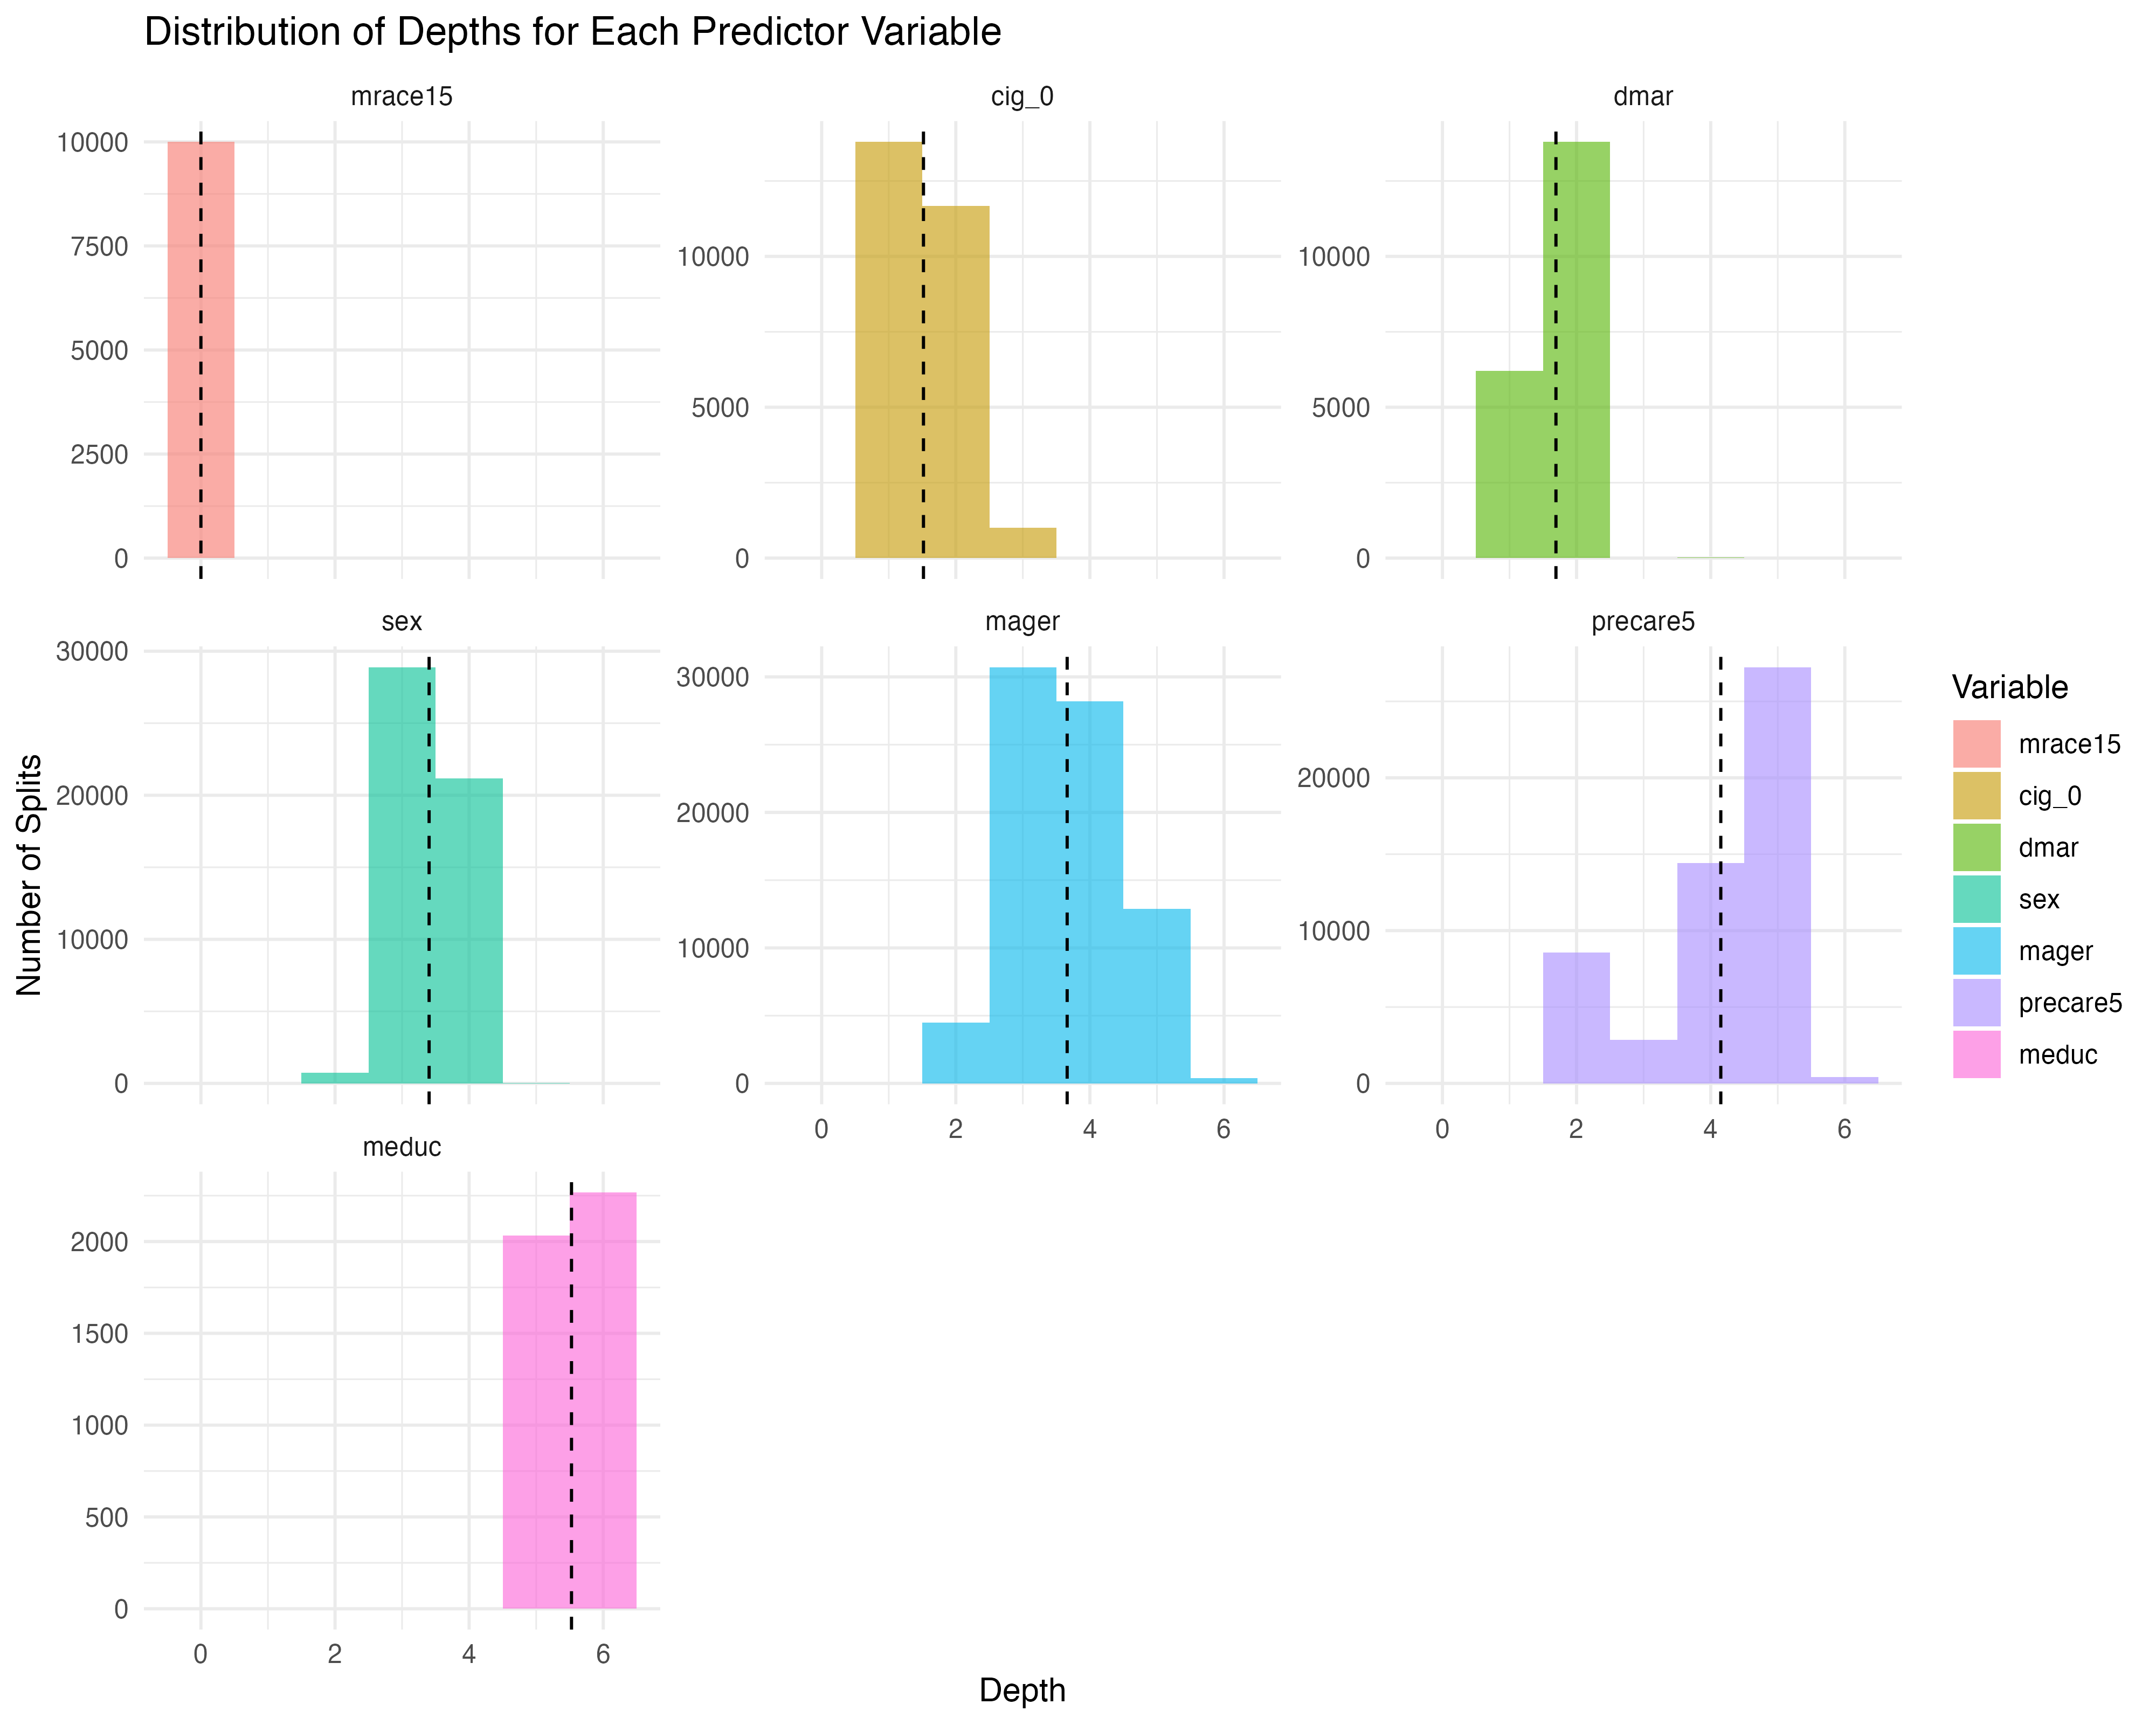
\includegraphics[width=1.0\textwidth]{chapters/chapter3/figures/boot/depth_distributions.png}
    \caption{Full model: Distribution of variable depths across the ensemble. Each panel shows a histogram indicating how frequently a given variable appears at each tree depth, where depth 0 corresponds to the root node. Variables closer to the root are generally more important in the model.}
    \label{fig:var-depth-distributions-full}
\end{figure}

% Depth distributions — LBW-only model
\begin{figure}[H]
    \centering
    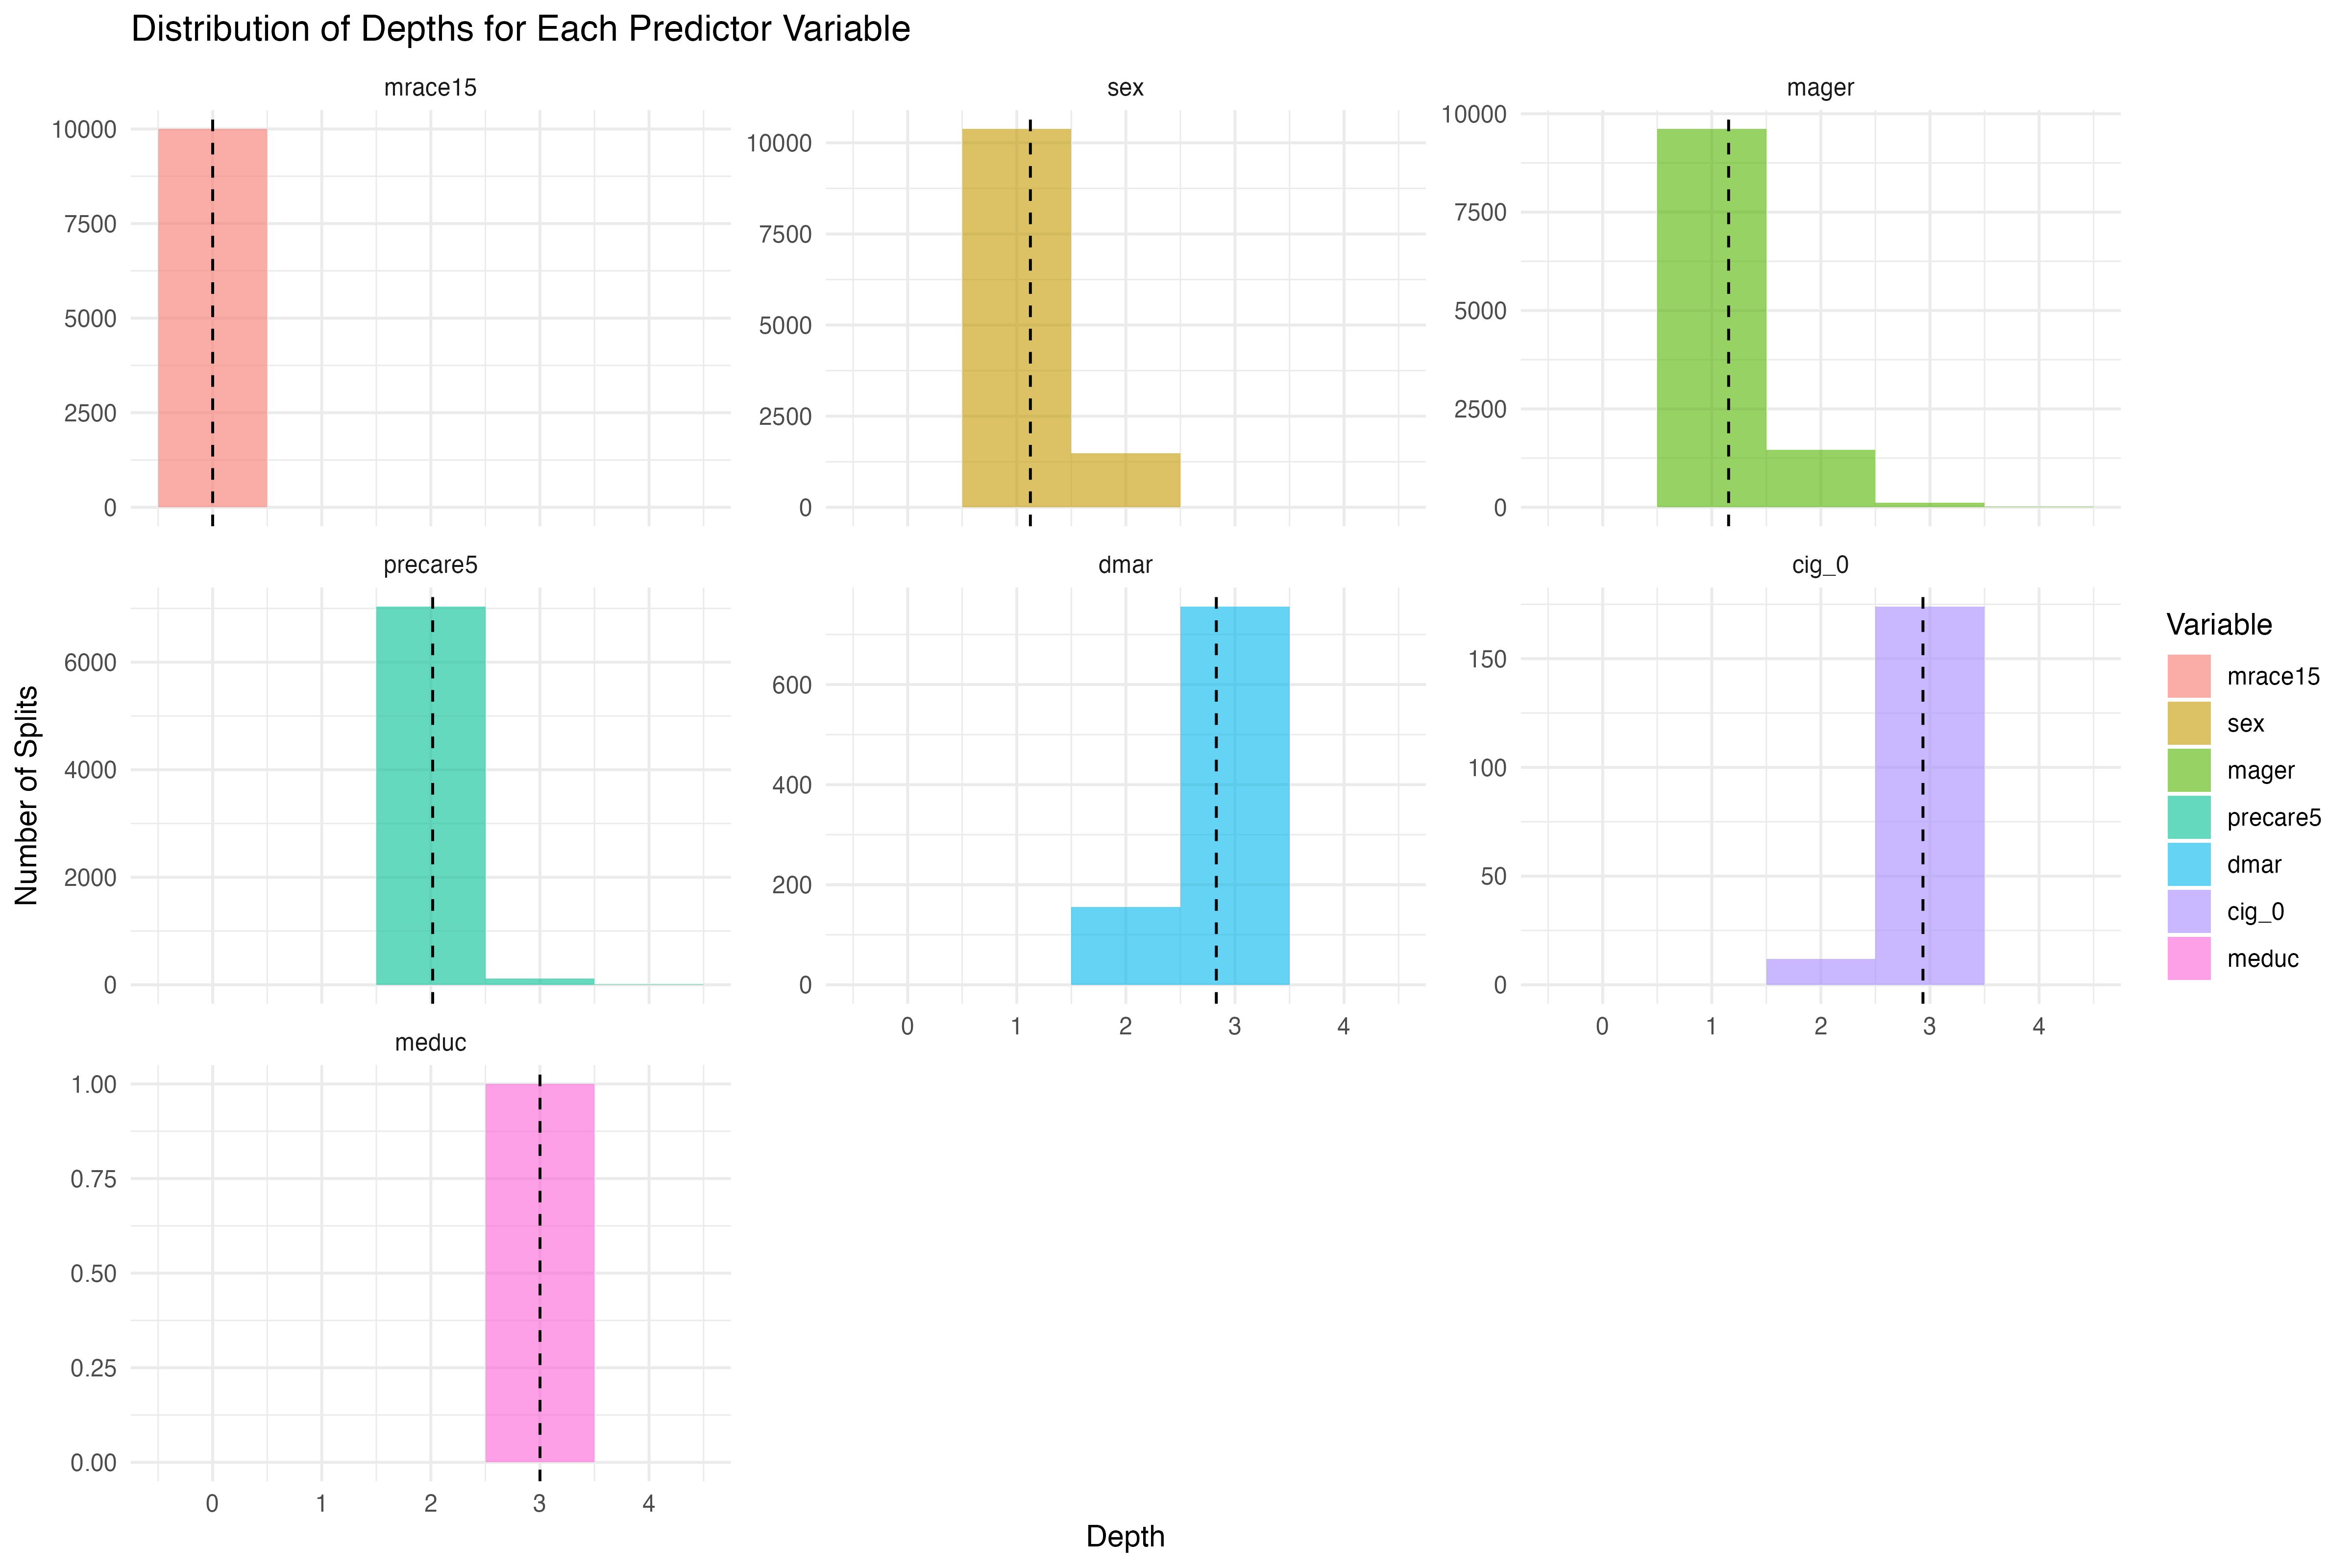
\includegraphics[width=1.0\textwidth]{chapters/chapter3/figures/boot/depth_distributions_2.png}
        \caption{LBW-only model: Distribution of variable depths across the ensemble. Each panel shows a histogram indicating how frequently a given variable appears at each tree depth, where depth 0 corresponds to the root node. Variables closer to the root are generally more important in the model.}
    \label{fig:var-depth-distributions-lbw}
\end{figure}


\chapter{Conclusion \& Future Work}
\label{chap:conclusion}

This study introduces a Bayesian tree-based methodology to investigating determinants of LBW using a nationally representative dataset. By the integration of the DM likelihood into the CART framework, the model addresses both data scarcity in rare outcome classes, with addressing the need for a more flexible and interpretable modeling structure. Using historic data, the quantiles inform the priors binning procedure, creating the necessary birth-weight categories. The quantile-based categories enable the the informed prior to represent subtle gradients in the LBW-region, and enabling detection of distributional shifts given a set of predictors. Additionally, the proposed bootstrap methodology handles the consolidated counts data, while the results yield stable and reliable estimates across the ensemble. 

A consistent theme in this project is that maternal race, marital status, and smoking status were dominant indicators of LBW risk. Furthermore, the restricted LBW-only model shifted the focus from socioeconomic and demographic predictors to biological and behavior-based variables. Such variables include maternal age, infant gender, and prenatal care. Note that these findings align with epidemiological literature, demonstrating the utility of our proposed modeling framework to extract and interpret clinically relevant rules from high-dimensional data. 

However, the present analysis is bounded by a constrained set of binary predictors and reductionist encoding of sociodemographic and behavioral traits. In further analysis, clinically relevant information could be utilized instead of discarded by encoding predictors into binary. Further, the race predictor currently represents a coarse proxy of demographic and socioeconomic conditions in further studies should refine this important predictor to capture more social and cultural dimensions. The most natural next step is enhancing the data with a richer predictor set of maternal-infant health and environmental indicators. Promising health related variables include: history of hypertension \parencite{hypertension_lbw}, diabetes \parencite{diabetes_lbw}, BMI \parencite{bmi_lbw} , mental health \parencite{mental_lbw}, and prior pregnancy complications \parencite{prior_lbw}. Including these variables could enhance the model's ability to further classify at-risk subgroups, since they are all known to affect fetal growth. Incorporating environmental and contextual variables can expand the model's scope and abilities. Structural determinant such as air quality metrics, neighborhood crime rates, housing conditions, food accessibility, and proximity to prenatal services may interact with biological and behavioral risks in meaningful ways. Their inclusion would support a more holistic understanding of LBW outcomes. Also, the temporal trends of any of these variables is worth while to investigate due to the consistent annual reporting of the natality dataset.

Moreover, this modeling framework has the potential to be enhanced as a practical tool for clinical triage or public health screening. Future work should focus on adapting the modeling framework into a practitioner-friendly risk calculator suitable for intake assessments or integration into electronic health records. This would significantly enhance accessibility for health practitioners and support early identification of at-risk pregnancies. 

This work contributes a flexible and interpretable modeling approach for modeling LBW determinants and lays the foundation for future interdisciplinary research that intersects statistical modeling, clinical practice, and public health policy. Expanding the set of predictors and translating the model into operational tools would be critical steps toward leveraging these insights into actionable health interventions.


% Bibliography
\begin{sloppypar}
    \printbibliography[heading=bibintoc,title=References]
\end{sloppypar}

% % Appendices
% \appendix
% % Main appendix file that includes all other appendices
\appendix
\chapter{Additional Material}
\label{app:appendices}

% Include individual appendix files
\section{Additional Material for Chapter 2}
\label{app:chapter2}

\section{Additional Material for Chapter 3}
\label{app:chapter3}


\end{document}
